\chapter{Memorization and Generalization}\label{ch:generalization}

\begin{chapterintro}
Picture two students preparing for a physics final. The first collects every past exam paper and memorizes every answer, word for word. The second works through the same papers but tries to understand why each answer is what it is. On the past papers both score 100\%. You cannot tell them apart by testing them on questions they have already seen. You can tell them apart instantly by giving them a question neither has seen.

This chapter turns that observation into a working method. You will learn what it means for a fitted model to ``learn'' something, how to split data into a part you fit and a part you hold back, why every claim of skill must be measured against a reference prediction that knows nothing (the \emph{null}), why a model with enough adjustable parameters can reproduce any data set and therefore proves nothing by doing so, and how the arrangement of training and test points (above, below, or interleaved) changes what a test measures. We will also derive two results that are less obvious: a smooth interpolation between neighbors can be \emph{anticorrelated} with the truth when consecutive values are negatively correlated, and the best linear predictor built from the correlations (simple kriging) flips that sign.

Where this shows up in the paper: the paper's central negative result is precisely the distinction between memorizing and predicting. Its out-of-sample protocol (Sec.~II~C), the within-height splits (Sec.~II~C and Table~III), the twelve Hermitian configurations of Table~I, the memorization curves of Fig.~3, the interpolation-gap damage of Fig.~4, and the heuristic explanation and falsifiability standard of Sec.~VI all rest on the ideas of this chapter~\cite{soniR1}.
\end{chapterintro}

\begin{prerequisites}
\item Chapter~\ref{ch:linear-algebra}: vectors, matrices, rank, solving $Ax=b$, overdetermined and underdetermined systems.
\item Chapter~\ref{ch:least-squares}: linear least squares, the normal equations, the singular value decomposition (SVD), minimum-norm solutions of underdetermined systems, ridge regularization with filter factors $\sigma/(\sigma^2+\lambda\sigma_1^2)$, and the memorizing polynomial (running example RE4).
\item Chapter~\ref{ch:probability}: mean, variance, standard deviation, covariance, Pearson correlation and its range $[-1,1]$, rms, autocorrelation of a sequence, random seeds.
\item Chapter~\ref{ch:fitting}: the fit of a potential correction $\delta V(x)=\sum_k c_k\phi_k(x)$ to a list of levels, the sensitivity matrix $A_{nk}$, the damped least-squares step, and the coverage law $M\pi/L>2\sqrt E$.
\item Used with short reminders at the point of use: the smooth zeros $s_n$ and the local mean spacing $\gap_n$ (Chapter~\ref{ch:counting-zeros}); the Wigner surmise for unfolded spacings (Chapter~\ref{ch:level-statistics}); classical turning points and where a level feels the potential (Chapter~\ref{ch:wkb}); first-order perturbation theory (Chapter~\ref{ch:perturbation}); the bias-corrected targets (Chapter~\ref{ch:finite-differences}); the truncated explicit formula (Chapter~\ref{ch:explicit-formula}); almost-periodic sums and phase randomization (Chapters~\ref{ch:fourier-series} and~\ref{ch:fourier-transform}); bootstrap and surrogate controls (Chapter~\ref{ch:controls}, forward references only).
\item First-year physics: graphs, averages, and the idea of a measurement uncertainty.
\end{prerequisites}

%======================================================================
\section{What does a model learn?}\label{sec:generalization-learn}
% DYK-BEGIN
\begin{didyouknow}{The Horse Who Read Faces}
In the early 1900s a Berlin horse called Clever Hans seemed to do arithmetic, tapping out answers with his hoof. In 1907 the psychologist Oskar Pfungst showed that Hans was reading tiny, unconscious cues in the questioner's posture and face, and that he failed when the questioner did not know the answer. A model can score perfectly while learning something other than what you intended.
\end{didyouknow}
% DYK-END

\subsection{Data, models and parameters}

Every problem in this chapter has the same ingredients.

\begin{itemize}
\item \textbf{Data.} A list of pairs $(x_i,y_i)$, $i=1,\dots,n$. The $x_i$ are \emph{inputs} (a time, a position, an index) and the $y_i$ are \emph{targets} (the measured values we want to reproduce).
\item \textbf{A model.} A family of functions $f(x;\bm c)$, one function for each choice of the \emph{parameter vector} $\bm c=(c_0,c_1,\dots,c_{M-1})$. The integer $M$ is the number of parameters.
\item \textbf{Fitting} (also called \emph{training}). A rule that chooses $\bm c$ from the data, usually by making the errors $f(x_i;\bm c)-y_i$ small in the least-squares sense of Chapter~\ref{ch:least-squares}.
\end{itemize}

Here are four models we will meet again.

\begin{enumerate}
\item \emph{A straight line}: $f(x;\bm c)=c_0+c_1x$, with $M=2$.
\item \emph{A polynomial of degree $M-1$}: $f(x;\bm c)=c_0+c_1x+\dots+c_{M-1}x^{M-1}$.
\item \emph{A fitted potential} (Chapter~\ref{ch:fitting}). The input is a level index $n$. The parameters are the coefficients $c_k$ of a correction $\delta V(x)=\sum_{k=0}^{M-1}c_k\cos(k\pi x/L)$ added to the Wu--Sprung potential $V(x)$ in a box $[-L,L]$. The output $f(n;\bm c)=E_n(\bm c)$ is the $n$-th eigenvalue of the Hamiltonian $H=-d^2/dx^2+V(x)+\delta V(x)$ (units $\hbar=2m=1$). The targets are the heights $t_n$ of the zeta zeros (in practice the bias-corrected targets $\tilde t_n$ of Chapter~\ref{ch:finite-differences}).
\item \emph{The truncated explicit formula} (Chapter~\ref{ch:explicit-formula}). The output is the $n$-th root of $\Nsm(t)+\Nfl(t)=n-\tfrac12$, built from a list of primes. It has \emph{no} fitted parameters at all: $M=0$.
\end{enumerate}

\subsection{Two meanings of ``learning''}

When we say a fitted model has ``learned'' from data, we might mean either of two very different things.

\emph{Storing.} The model's parameters hold a copy of the data. A lookup table that lists the first 400 zeros reproduces them perfectly, yet nobody would say it has learned anything about where zero 401 is.

\emph{Capturing a rule.} The model has picked up the mechanism (or a good stand-in for it) that generates the data, so it can tell you about data it was never shown.

Fitting quality alone cannot separate these two. Both the lookup table and a correct physical law reproduce the training data. What separates them is the question the second student can answer and the first cannot: \emph{what happens at a point you did not fit?} This leads to the operational definition used throughout this book and in the paper.

\begin{center}
\fbox{\parbox{0.9\linewidth}{\textbf{Operational definition.} A fitted model has \emph{captured structure} (rather than stored data) to the extent that it predicts targets it was not shown better than a reference prediction that uses no information about them.}}
\end{center}

The paper states it this way: a model fitted to zeros $1,\dots,n_{\rm fit}$ ``has captured structure, rather than data, only to the extent that it predicts zeros it was not shown,'' and ``capture'' is ``predictive transfer to held-out zeros, measured by rms error and correlation relative to the model's own smooth baseline'' (Sec.~I)~\cite{soniR1}. The words ``rather than data'' are the memorizing student; the words ``relative to the model's own smooth baseline'' are the reference prediction, which we will call the \emph{null}.

\begin{checkpoint}
A friend fits a model with 500 parameters to 500 measured numbers and reports that every number is reproduced to six decimal places. Has the friend shown that the model has captured structure?
\end{checkpoint}
\checkanswer{No. With as many parameters as data points, an exact reproduction can be a disguised lookup table. Only a prediction of numbers that were not used in the fit, compared with a null, can show captured structure.}

\begin{keyideas}
\item A model is a family $f(x;\bm c)$; fitting chooses $\bm c$ from data.
\item Reproducing the fitted data cannot distinguish storing the data from capturing the rule that generated it.
\item Operationally, a model has captured structure only to the extent that it predicts unseen data better than a null.
\end{keyideas}

%======================================================================
\section{Training sets, test sets and two kinds of error}\label{sec:generalization-split}

\subsection{The split}

Divide the indices $\{1,\dots,n\}$ into two disjoint sets: a \emph{training set} $I_{\rm tr}$ and a \emph{test set} (also called the \emph{held-out set} or \emph{holdout}) $I_{\rm te}$. Fit the model using only the pairs with $i\in I_{\rm tr}$. Then, once and only once, evaluate the fitted model on $I_{\rm te}$.

\begin{itemize}
\item The \textbf{in-sample error} is the rms error on the training set,
\begin{equation}
E_{\rm in}=\left[\frac{1}{|I_{\rm tr}|}\sum_{i\in I_{\rm tr}}\bigl(f(x_i;\bm c)-y_i\bigr)^2\right]^{1/2},
\label{eq:generalization-Ein}
\end{equation}
where $|I_{\rm tr}|$ is the number of indices in the training set.
\item The \textbf{out-of-sample (OOS) error} is the rms error on the test set,
\begin{equation}
E_{\rm out}=\left[\frac{1}{|I_{\rm te}|}\sum_{i\in I_{\rm te}}\bigl(f(x_i;\bm c)-y_i\bigr)^2\right]^{1/2}.
\label{eq:generalization-Eout}
\end{equation}
\item The \textbf{generalization gap} is $E_{\rm out}-E_{\rm in}$.
\end{itemize}

Recall from Chapter~\ref{ch:probability} that ``rms'' means \emph{root mean square}: square each error, average the squares, take the square root. An rms error has the same units as the targets.

The one rule that makes the test meaningful is this: \textbf{nothing about the test targets may influence any choice made before scoring.} That includes the coefficients $\bm c$, the number of parameters $M$, any regularization strength, the number of optimizer iterations, and the decision of which runs to report. If you look at the test error, change $M$, and look again, the test set has quietly become part of the training set.

\begin{sample}{Train, test and null on four points}
A quantity is measured at $t=1,2,3,4$ (arbitrary units) with results $y=1.0,\,1.4,\,1.2,\,1.3$. Fit on the first three points only and predict the fourth. Compare three models: a constant $f=c_0$, a line $f=c_0+c_1t$, and a quadratic $f=c_0+c_1t+c_2t^2$. Treat the constant model as the null (``predict the typical value'').

Step 1: Constant model. Least squares for a constant gives the mean (Chapter~\ref{ch:least-squares}): $c_0=(1.0+1.4+1.2)/3=1.2$. Residuals are $-0.2,\,+0.2,\,0$, so
\[
E_{\rm in}=\sqrt{\frac{0.04+0.04+0}{3}}=\sqrt{0.02667}=0.1633.
\]
Prediction at $t=4$: $1.2$; error $\abs{1.3-1.2}=0.1$.

Step 2: Line. With $\bar t=2$ and $\bar y=1.2$, the least-squares slope is
\[
c_1=\frac{\sum(t_i-\bar t)(y_i-\bar y)}{\sum(t_i-\bar t)^2}=\frac{(-1)(-0.2)+(0)(0.2)+(1)(0)}{1+0+1}=\frac{0.2}{2}=0.1,
\]
so $f(t)=1.2+0.1(t-2)$. Fitted values $1.1,\,1.2,\,1.3$; residuals $-0.1,\,+0.2,\,-0.1$;
\[
E_{\rm in}=\sqrt{\frac{0.01+0.04+0.01}{3}}=\sqrt{0.02}=0.1414.
\]
Prediction at $t=4$: $1.2+0.1(2)=1.4$; error $\abs{1.3-1.4}=0.1$.

Step 3: Quadratic. Three parameters, three points: the quadratic passes through all of them. Write $f(t)=1.4+b(t-2)+a(t-2)^2$ (so that $f(2)=1.4$). Then $f(1)=1.4-b+a=1.0$ and $f(3)=1.4+b+a=1.2$. Adding the two equations: $2.8+2a=2.2$, so $a=-0.3$. Subtracting: $2b=0.2$, so $b=0.1$. In-sample error: $E_{\rm in}=0$. Prediction at $t=4$:
\[
f(4)=1.4+0.1(2)-0.3(2)^2=1.4+0.2-1.2=0.4,
\]
error $\abs{1.3-0.4}=0.9$.

Step 4: Compare (Table~\ref{tab:generalization-four}). The quadratic has the best in-sample error (zero) and by far the worst test error.

\[
\boxed{E_{\rm in}:\ 0.163,\ 0.141,\ 0;\qquad E_{\rm out}:\ 0.1,\ 0.1,\ 0.9}
\]
\end{sample}

\begin{table}[htbp]\centering
\caption{The three models of the Sample Problem ``Train, test and null on four points''. More parameters always lower (or keep) the in-sample error; they need not lower the out-of-sample error.}
\label{tab:generalization-four}
\begin{tabular}{lccc}
\toprule
model & parameters $M$ & $E_{\rm in}$ & $E_{\rm out}$ (point $t=4$) \\
\midrule
constant (null) & 1 & 0.163 & 0.1 \\
line & 2 & 0.141 & 0.1 \\
quadratic & 3 & 0 & 0.9 \\
\bottomrule
\end{tabular}
\end{table}

Why does in-sample error never increase as we go from constant to line to quadratic? Because the models are \emph{nested}: every constant is a line with $c_1=0$, and every line is a quadratic with $c_2=0$. The least-squares quadratic minimizes the error over a set that contains every line, so its minimum cannot be larger than the best line's. This argument holds for any nested family, including cosine expansions $\delta V$ with growing $M$.

\begin{pitfall}
Reporting only the in-sample error of a flexible model. A falling in-sample error as $M$ grows is guaranteed by nesting, whether or not the model is learning anything. It is a statement about the size of the family, not about the data.
\end{pitfall}

\begin{pitfall}
Tuning on the test set. If you try $M=200,400,600$ and report whichever gives the best test error, the reported number is biased downward, because the test set was used to make a choice. The cure is a third split: choose settings on a \emph{validation} part of the training data, then score the test set once. The paper does exactly this for its fitted sinusoidal controls: ``Ridge strength and $K$ are chosen by a forward split inside the training window (first 75\% fit, last 25\% validate)'' (Sec.~II~D).
\end{pitfall}

\begin{checkpoint}
In the four-point Sample Problem, suppose we had fitted the quadratic to all four points with least squares (four points, three parameters). Would the resulting error at $t=4$ be a legitimate out-of-sample error?
\end{checkpoint}
\checkanswer{No. The point $t=4$ would then be part of the training set; its residual would be an in-sample error.}

\begin{keyideas}
\item Split indices into disjoint training and test sets; fit on the first, score once on the second.
\item $E_{\rm in}$ can only fall (or stay the same) as a nested family grows; $E_{\rm out}$ can rise.
\item No test target may influence any choice made before scoring.
\end{keyideas}

%======================================================================
\section{The null model: every claim is relative}\label{sec:generalization-null}

\subsection{Why a reference is needed}

Suppose someone tells you their model predicts held-out zeros ``to 0.3 mean spacings.'' Is that good? You cannot say until you know how well a prediction that \emph{knows nothing about the fluctuations} would do. If that trivial prediction already achieves 0.26, then 0.3 is worse than knowing nothing.

\textbf{Definition.} The \emph{null model} for a prediction task is the best prediction available without using the information the model claims to capture. A model shows \emph{skill} only if it beats the null on held-out data.

\subsection{The null for the zeta zeros}

Recall from Chapter~\ref{ch:counting-zeros} the smooth counting function $\Nsm(t)=\frac{t}{2\pi}\log\frac{t}{2\pi}-\frac{t}{2\pi}+\frac78$ (paper Eq.~(1)), the \emph{smooth zeros} $s_n$ defined by $\Nsm(s_n)=n-\tfrac12$, and the \emph{local mean spacing} $\gap_n=ds_n/dn=2\pi/\log(s_n/2\pi)$. The smooth zeros are where the zeros would sit if they were perfectly evenly spread according to their average density. The true zero $t_n$ deviates from $s_n$; we measure that deviation in units of the local spacing,
\begin{equation}
d_n=\frac{t_n-s_n}{\gap_n},
\label{eq:generalization-dn}
\end{equation}
called the \emph{fluctuation} of zero $n$ (\texttt{qmnt.fluct}).

A predictor produces predicted heights $\hat t_n$, hence predicted fluctuations $\hat d_n=(\hat t_n-s_n)/\gap_n$. Subtracting,
\begin{equation}
\hat d_n-d_n=\frac{\hat t_n-s_n}{\gap_n}-\frac{t_n-s_n}{\gap_n}=\frac{\hat t_n-t_n}{\gap_n},
\label{eq:generalization-diff}
\end{equation}
so the error in the fluctuation equals the error in the height, in mean spacings. Over a held-out set $H$ the paper reports
\begin{equation}
\mathrm{rms}=\left[\frac{1}{|H|}\sum_{n\in H}\left(\frac{\hat t_n-t_n}{\gap_n}\right)^2\right]^{1/2},
\qquad
\mathrm{corr}=\text{Pearson correlation of }\{\hat d_n\}\text{ and }\{d_n\},\ n\in H.
\label{eq:generalization-score}
\end{equation}

The null predicts ``no fluctuation'': $\hat t_n=s_n$, so $\hat d_n=0$ and, by Eq.~\eqref{eq:generalization-diff}, the null rms is simply the rms of the true fluctuations:
\begin{equation}
\mathrm{rms}_{\rm null}=\left[\frac{1}{|H|}\sum_{n\in H}d_n^2\right]^{1/2}.
\label{eq:generalization-null}
\end{equation}
The correlation of the null is undefined (a constant has no variance), which is natural: the null makes no claim about the pattern.

For the fitted potential, the paper's null is the unperturbed Wu--Sprung potential itself, and fluctuations are measured relative to its levels. On the principal holdout (zeros 401--500) the two nulls give the same number, $0.2631$, which is why the operator and the explicit-formula comparisons can share one baseline (Sec.~II~C).

\begin{pycode}
import numpy as np, qmnt
t = qmnt.zeros(500)              # t_1 ... t_500
n = np.arange(401, 501)          # the principal holdout (RE5)
d = qmnt.fluct(t[400:500], n)    # true fluctuations in mean spacings
print("null rms on 401-500:", qmnt.rms(d))
\end{pycode}

\subsection{A skill ratio}

A convenient summary is the ratio of a model's held-out rms to the null rms,
\begin{equation}
\text{ratio}=\frac{\mathrm{rms}_{\rm model}}{\mathrm{rms}_{\rm null}},\qquad \text{skill}=1-\text{ratio}.
\label{eq:generalization-skill}
\end{equation}
A ratio below 1 (positive skill) means the model beats the null; a ratio above 1 (negative skill) means it does harm.

\begin{sample}{The null on RE5 and two predictions measured against it}
(a) Compute the null rms on zeros 401--500 with \texttt{qmnt}. (b) The paper's Table~I reports held-out rms $0.369$ for the scale-1 cosine fit with $M=400$ trained on zeros 1--400, and Table~V reports $0.074$ for the six-prime explicit formula on the same holdout. Compute the ratio and skill of each, using the paper's rounded null $0.263$.

Step 1: Run the listing above. It evaluates Eq.~\eqref{eq:generalization-null} with $d_n$ from Eq.~\eqref{eq:generalization-dn} and prints $0.2631$, matching the paper's value (Sec.~II~C and the key anchors of App.~A).

Step 2: Fitted operator: ratio $=0.369/0.263=1.403$, skill $=1-1.403=-0.403$.

Step 3: Six-prime formula: ratio $=0.074/0.263=0.281$, skill $=1-0.281=0.719$.

\[
\boxed{\mathrm{rms}_{\rm null}=0.2631;\quad \text{operator: ratio }1.40\ (\text{skill }-0.40);\quad \text{formula: ratio }0.281\ (\text{skill }+0.72)}
\]
The fitted operator is about 40\% \emph{worse} than predicting no fluctuation at all; the formula removes most of the null error. (You can reproduce the formula's numbers yourself with \texttt{qmnt.oracle\_zeros} and \texttt{qmnt.score}; Problem~30 does this for one prime.)
\end{sample}

\subsection{rms and correlation measure different things}

Why does the paper always report \emph{two} numbers? Because a prediction can have the right shape and the wrong size, or the right size and no shape. Let us make that precise.

Suppose that over the held-out set the true fluctuations $d$ have mean zero and standard deviation $\sigma$, and the predicted fluctuations $\hat d$ have mean zero, standard deviation $a\sigma$ (so $a$ is the \emph{amplitude ratio}) and correlation $\rho$ with $d$. Recall from Chapter~\ref{ch:probability} that $\mathrm{Cov}(\hat d,d)=\rho\,(a\sigma)(\sigma)$. Because both means are zero, the average of a square is a variance and the average of a product is a covariance. The mean squared error is
\begin{align}
\mathrm{MSE}&=\overline{(\hat d-d)^2}\notag\\
&=\overline{\hat d^{\,2}}-2\,\overline{\hat d\,d}+\overline{d^2}&&\text{(expand the square)}\notag\\
&=a^2\sigma^2-2\rho a\sigma^2+\sigma^2&&\text{(zero means)}\notag\\
&=\sigma^2\bigl(1+a^2-2\rho a\bigr).
\end{align}
The null has $\mathrm{MSE}=\sigma^2$, so
\begin{equation}
\frac{\mathrm{rms}_{\rm model}}{\mathrm{rms}_{\rm null}}=\sqrt{1+a^2-2\rho a}.
\label{eq:generalization-ratio}
\end{equation}

Three consequences follow directly.
\begin{enumerate}
\item If $\rho\le0$, every $a>0$ makes the ratio exceed 1: an uncorrelated (or anticorrelated) prediction with any nonzero amplitude is worse than the null.
\item For fixed $\rho$, the ratio is smallest when $\frac{d}{da}(1+a^2-2\rho a)=2a-2\rho=0$, that is $a=\rho$. The minimum value is $\sqrt{1+\rho^2-2\rho^2}=\sqrt{1-\rho^2}$. No rescaling of a prediction can beat $\sqrt{1-\rho^2}$.
\item A prediction with positive correlation can still be worse than the null if its amplitude is too large: the ratio exceeds 1 when $a^2-2\rho a>0$, i.e.\ when $a>2\rho$.
\end{enumerate}
The assumption of zero means is an idealization; a constant offset between $\hat d$ and $d$ adds its square to the MSE and makes things worse still.

\begin{sample}{Uncorrelated output always adds error}
The paper reports that the fitted Hermitian models ``emit fluctuations of $0.16$--$0.62\times$ the true amplitude that are uncorrelated with truth'' (Sec.~III). Using Eq.~\eqref{eq:generalization-ratio} with null $0.263$, find the held-out rms of a prediction with (a) $a=0.62$, $\rho=0$; (b) $a=0.62$, $\rho=-0.07$; (c) $a=0.16$, $\rho=0$.

Step 1: (a) $\sqrt{1+0.62^2}=\sqrt{1.3844}=1.1766$; rms $=1.1766\times0.263=0.309$.

Step 2: (b) $\sqrt{1+0.3844-2(-0.07)(0.62)}=\sqrt{1.3844+0.0868}=\sqrt{1.4712}=1.2129$; rms $=1.2129\times0.263=0.319$.

Step 3: (c) $\sqrt{1+0.0256}=1.0127$; rms $=0.266$.

\[
\boxed{\text{(a) }0.309,\quad\text{(b) }0.319,\quad\text{(c) }0.266}
\]
All three are worse than the null $0.263$. This is an idealized calculation, not a reconstruction of any table row: real held-out errors (for example $0.369$ in Table~I) also include offsets and amplitude variations that Eq.~\eqref{eq:generalization-ratio} ignores. The lesson is general: output that is uncorrelated with the truth can only add error.
\end{sample}

\begin{checkpoint}
A prediction has correlation $\rho=+0.5$ with the truth but twice the true amplitude ($a=2$). Is it better or worse than the null?
\end{checkpoint}
\checkanswer{Worse: the ratio is $\sqrt{1+4-2(0.5)(2)}=\sqrt3=1.73$. Since $a=2>2\rho=1$, positive correlation does not save it.}

\begin{keyideas}
\item The null is the best prediction that uses none of the information a model claims to capture; skill means beating it on held-out data.
\item For the zeros, the null is $\hat t_n=s_n$ (or the unperturbed potential's levels), with rms equal to the rms of the true fluctuations, $0.2631$ on zeros 401--500.
\item $\mathrm{rms}_{\rm model}/\mathrm{rms}_{\rm null}=\sqrt{1+a^2-2\rho a}$: correlation $\rho$ measures shape, amplitude ratio $a$ measures size; uncorrelated output always hurts, and the best possible ratio at correlation $\rho$ is $\sqrt{1-\rho^2}$.
\end{keyideas}

%======================================================================
\section{Overfitting and capacity: the memorizing polynomial}\label{sec:generalization-overfit}

\subsection{RE4 revisited}

Recall running example RE4 from Chapter~\ref{ch:least-squares}: a few noisy samples of $\sin t$ fitted by a polynomial. Figure~\ref{fig:generalization-polyfit} shows ten such samples on $0\le t\le2\pi$ fitted by polynomials of degree 1, 3 and 9. The degree-9 polynomial has ten coefficients and passes exactly through all ten points. Inside the training range it wiggles to chase the noise; just beyond it, it shoots off.

\begin{figure}[htbp]\centering
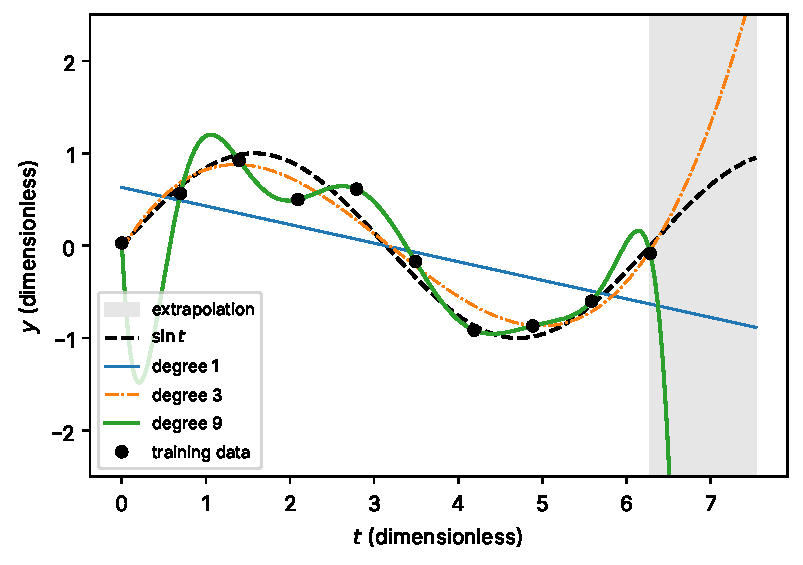
\includegraphics[width=0.85\linewidth]{figs/generalization_polyfit.pdf}
\caption{Running example RE4. Ten noisy samples (dots) of $\sin t$ (dashed) on $0\le t\le2\pi$, fitted by least-squares polynomials of degree 1, 3 and 9. The degree-9 polynomial has as many coefficients as points and passes through every one of them; in the shaded extrapolation region $t>2\pi$ it departs rapidly from the truth. Horizontal axis: $t$ (dimensionless); vertical axis: $y$ (dimensionless).}
\label{fig:generalization-polyfit}
\end{figure}

\textbf{Definition.} A fit \emph{overfits} when it lowers its in-sample error by adapting to features of the training data that do not recur in new data (noise, or accidents of the particular sample), so that its out-of-sample error rises.

Figure~\ref{fig:generalization-errorcurve} shows the error curves for a larger version of RE4 (15 training points). The in-sample error falls with degree, as nesting guarantees. The out-of-sample error behaves differently for test points inside the training range and for test points beyond it. Inside the range (squares), the test error is large at degrees 0 to 2, which cannot follow a full period of the sine. It reaches its minimum at a moderate degree (between 3 and 12 for the data of the listing below) and is larger again at degree 14, where the fit chases the noise. Beyond the range (triangles), the error grows rapidly with degree: at degree 14 it is more than ten times its value at degree 3.

\begin{figure}[htbp]\centering
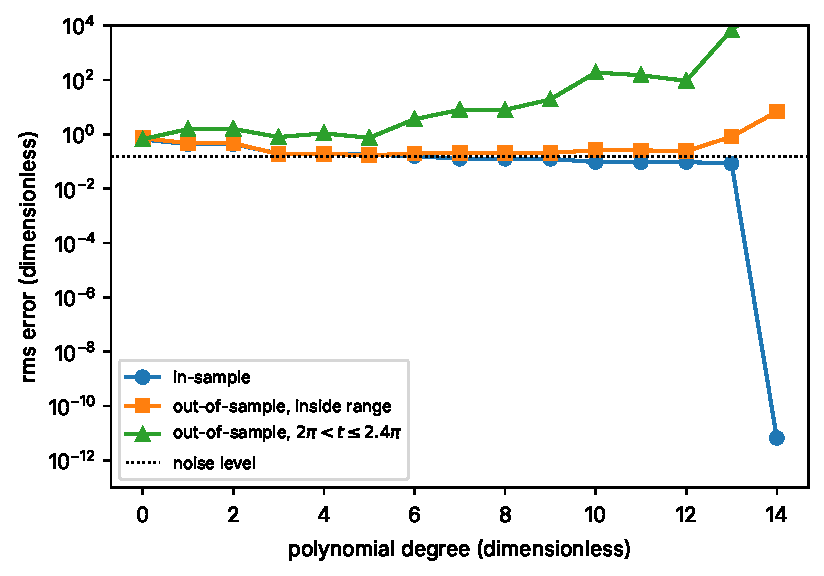
\includegraphics[width=0.85\linewidth]{figs/generalization_errorcurve.pdf}
\caption{Error versus polynomial degree for RE4 with 15 noisy training points on $0\le t\le2\pi$ (noise standard deviation 0.15). In-sample rms (circles) never increases with degree because the models are nested, and falls to a negligible value (below $10^{-6}$) at degree 14, where the fit interpolates. Out-of-sample rms is shown for fresh noisy points inside the training range (squares, interpolation) and for points with $2\pi<t\le2.4\pi$ (triangles, extrapolation). Dotted line: the noise level. Vertical axis logarithmic; all quantities dimensionless.}
\label{fig:generalization-errorcurve}
\end{figure}

\begin{pycode}
import numpy as np
rng = np.random.default_rng(3)
t_tr = np.linspace(0, 2*np.pi, 15)
y_tr = np.sin(t_tr) + 0.15*rng.standard_normal(15)
t_in = rng.uniform(0, 2*np.pi, 200)            # interpolation test
t_out = np.linspace(2*np.pi, 2.4*np.pi, 50)    # extrapolation test
y_in = np.sin(t_in) + 0.15*rng.standard_normal(200)
y_out = np.sin(t_out) + 0.15*rng.standard_normal(50)
rms = lambda e: np.sqrt(np.mean(e**2))
for deg in range(15):
    p = np.polynomial.Polynomial.fit(t_tr, y_tr, deg)
    print(deg, rms(p(t_tr)-y_tr), rms(p(t_in)-y_in), rms(p(t_out)-y_out))
\end{pycode}

\begin{sample}{Interpolation works, extrapolation fails}
Take three noisy samples of $\sin t$: $(0,\,0.1)$, $(\pi/2,\,0.9)$, $(\pi,\,0.1)$. (The true values are $0,1,0$; the noise is $+0.1,-0.1,+0.1$.) Fit the unique quadratic through them. Predict at $t=\pi/4$ (inside the range) and at $t=3\pi/2$ (outside). Compare with the truth and with the null ``predict zero''.

Step 1: The data are symmetric about $t=\pi/2$, so try $q(t)=0.9-a(t-\pi/2)^2$, which already passes through the middle point. At $t=0$: $0.9-a\pi^2/4=0.1$, so $a=0.8\times4/\pi^2=3.2/\pi^2=0.324$. By symmetry $q(\pi)=0.1$ too, so the quadratic fits all three points: $E_{\rm in}=0$.

Step 2: Interpolation, $t=\pi/4$: $(t-\pi/2)^2=\pi^2/16$, so $q=0.9-\frac{3.2}{\pi^2}\cdot\frac{\pi^2}{16}=0.9-0.2=0.7$. True value $\sin(\pi/4)=0.7071$. Error $0.0071$.

Step 3: Extrapolation, $t=3\pi/2$: $(t-\pi/2)^2=\pi^2$, so $q=0.9-3.2=-2.3$. True value $\sin(3\pi/2)=-1$. Error $\abs{-1-(-2.3)}=1.3$. The null ``predict zero'' has error $\abs{-1-0}=1$.

Step 4: For comparison, the least-squares line through the three points has slope 0 (the data are symmetric) and intercept equal to the mean $1.1/3=0.3667$; its error at $3\pi/2$ is $1.3667$.

\[
\boxed{\text{at }\pi/4:\ \text{error }0.0071;\qquad\text{at }3\pi/2:\ \text{error }1.3\ (\text{null }1)}
\]
The same fitted curve is excellent between its training points and worse than the null beyond them. Whether a fit generalizes depends on \emph{where} you ask.
\end{sample}

\subsection{Capacity and saturation}

How much a model family can fit is called its \emph{capacity}. For a model that is linear in its parameters, $f(x;\bm c)=\sum_{k}c_k\phi_k(x)$, capacity has a precise meaning. Arrange the training inputs into the \emph{design matrix} $X_{\rm tr}$ with entries $(X_{\rm tr})_{ik}=\phi_k(x_i)$, $i\in I_{\rm tr}$; then the vector of predictions on the training set is $X_{\rm tr}\bm c$. Recall from Chapter~\ref{ch:linear-algebra} that the \emph{rank} of a matrix is the number of linearly independent columns (equivalently, rows). The rank of $X_{\rm tr}$ is the number of independent patterns of training values the model can produce.

\textbf{Definition.} The model is \emph{saturated} on a training set when the rank of $X_{\rm tr}$ equals the number of training points $n_{\rm tr}$. A saturated model can fit \emph{any} training targets exactly: rank $n_{\rm tr}$ means the columns of $X_{\rm tr}$ span all of $\mathbb R^{n_{\rm tr}}$, so every target vector $\bm y_{\rm tr}$ is a combination $X_{\rm tr}\bm c$ of them. A necessary condition is $M\ge n_{\rm tr}$.

For the fitted potential, the model is not linear in $\bm c$: the levels $E_n(\bm c)$ depend on $\bm c$ through an eigenvalue problem. Recall from Chapters~\ref{ch:perturbation} and~\ref{ch:fitting} that for small changes it is linear to first order, $\delta E_n\approx\sum_kA_{nk}c_k$ with $A_{nk}=\int|\psi_n|^2\phi_k\,dx$. The sensitivity matrix $A$ plays the role of $X$, and ``$M\ge$ number of training levels'' is the warning sign of saturation. (The paper uses the letter $A$ also for a non-Hermitian operator in Sec.~II~E; here it always means the sensitivity matrix.)

\subsection{A saturated model's predictions are not constrained by its data}

Here is the central mathematical fact of this chapter.

\medskip\noindent\textbf{Result (proved).} Let a linear model have training design matrix $X_{\rm tr}$ ($n_{\rm tr}\times M$) and test design matrix $X_{\rm te}$ ($n_{\rm te}\times M$). Suppose the stacked matrix $X=\begin{pmatrix}X_{\rm tr}\\X_{\rm te}\end{pmatrix}$, of size $(n_{\rm tr}+n_{\rm te})\times M$, has rank $n_{\rm tr}+n_{\rm te}$. Then for \emph{any} training targets $\bm y_{\rm tr}$ and \emph{any} vector $\bm z$ of desired test predictions, there is a parameter vector $\bm c$ with $X_{\rm tr}\bm c=\bm y_{\rm tr}$ and $X_{\rm te}\bm c=\bm z$.

\emph{Proof.} The rank of $X$ equals its number of rows, so its columns span $\mathbb R^{n_{\rm tr}+n_{\rm te}}$ (Chapter~\ref{ch:linear-algebra}). Hence the stacked vector $\begin{pmatrix}\bm y_{\rm tr}\\ \bm z\end{pmatrix}$ is a combination of the columns: there is $\bm c$ with $X\bm c=\begin{pmatrix}\bm y_{\rm tr}\\ \bm z\end{pmatrix}$. Reading off the top $n_{\rm tr}$ rows gives $X_{\rm tr}\bm c=\bm y_{\rm tr}$; the bottom $n_{\rm te}$ rows give $X_{\rm te}\bm c=\bm z$. $\square$

In words: among the parameter vectors that fit the training data \emph{perfectly}, there is one that predicts any held-out values you like. The training data cannot select among them. Whatever the model ends up predicting on the test set is decided by something other than the data: the optimizer's starting point, its step rule, a regularizer, the choice of basis. That ``something other'' is called the model's \emph{inductive bias}, and we return to it in Sec.~\ref{sec:generalization-bias}.

\begin{sample}{Infinitely many perfect fits, one chosen by the minimum norm}
Fit $f(t)=c_0+c_1t+c_2t^2$ to two points, $f(0)=1$ and $f(1)=2$, and predict at $t=2$. (a) Describe all exact fits and their predictions. (b) Find the minimum-norm exact fit (Chapter~\ref{ch:least-squares}) and its prediction.

Step 1: The conditions are $c_0=1$ and $c_0+c_1+c_2=2$, so $c_1+c_2=1$, i.e.\ $c_1=1-c_2$ with $c_2$ free.

Step 2: Prediction at $t=2$: $f(2)=c_0+2c_1+4c_2=1+2(1-c_2)+4c_2=3+2c_2$. As $c_2$ ranges over all real numbers, so does the prediction. The two data points say nothing about $f(2)$.

Step 3: Minimum norm. With $c_0=1$ fixed, minimize $c_0^2+c_1^2+c_2^2=1+(1-c_2)^2+c_2^2$. The derivative with respect to $c_2$ is $-2(1-c_2)+2c_2=4c_2-2$, which vanishes at $c_2=\tfrac12$; then $c_1=\tfrac12$. So $\bm c=(1,\tfrac12,\tfrac12)$.

Step 4: Check with the formula of Chapter~\ref{ch:least-squares}, $\bm c=X_{\rm tr}^\top(X_{\rm tr}X_{\rm tr}^\top)^{-1}\bm y_{\rm tr}$. Here $X_{\rm tr}=\begin{pmatrix}1&0&0\\1&1&1\end{pmatrix}$, $X_{\rm tr}X_{\rm tr}^\top=\begin{pmatrix}1&1\\1&3\end{pmatrix}$, whose inverse is $\frac12\begin{pmatrix}3&-1\\-1&1\end{pmatrix}$. Then $(X_{\rm tr}X_{\rm tr}^\top)^{-1}\bm y_{\rm tr}=\frac12\begin{pmatrix}3-2\\-1+2\end{pmatrix}=\begin{pmatrix}0.5\\0.5\end{pmatrix}$ and $X_{\rm tr}^\top\begin{pmatrix}0.5\\0.5\end{pmatrix}=\begin{pmatrix}1\\0.5\\0.5\end{pmatrix}$, as found.

Step 5: Prediction: $f(2)=1+2(0.5)+4(0.5)=4$.

\[
\boxed{f(2)=3+2c_2\ \text{for any }c_2;\qquad\text{minimum norm: }\bm c=(1,\tfrac12,\tfrac12),\ f(2)=4}
\]
A straight line through the two points would predict 3. The minimum-norm rule predicts 4, not because the data demand it, but because ``small coefficients'' is the rule we chose.
\end{sample}

\begin{checkpoint}
A cosine model with $M=400$ coefficients is fitted to 200 training levels. Is it necessarily saturated? What extra condition is needed?
\end{checkpoint}
\checkanswer{Not necessarily: $M\ge n_{\rm tr}$ is necessary but not sufficient. Saturation requires the (linearized) training sensitivity matrix to have rank 200, i.e.\ 200 independent level patterns among its columns.}

\begin{keyideas}
\item Overfitting: lowering in-sample error by fitting features that do not recur, at the cost of out-of-sample error.
\item Capacity of a linear model is the rank of its design matrix; it is saturated when that rank equals the number of training points, and then fits any targets exactly.
\item If training and test rows together have full row rank, exact training fits exist with \emph{any} test predictions; the data cannot choose, the inductive bias does.
\end{keyideas}

%======================================================================
\section{Interpolation, extrapolation and covariate shift}\label{sec:generalization-shift}
% DYK-BEGIN
\begin{didyouknow}{Two Million Wrong Answers}
In 1936 the \emph{Literary Digest} polled about 2.4 million people and predicted that Alf Landon would defeat Franklin Roosevelt. Roosevelt won in a landslide. The mailing lists, drawn largely from telephone directories and car registrations, did not represent all voters. George Gallup, with a far smaller sample, called the winner. A model built on one population can fail badly on another.
\end{didyouknow}
% DYK-END

\subsection{Where the test points lie}

The RE4 Sample Problem showed that the same fit can be good inside its training range and bad outside. We name the two situations.

\begin{itemize}
\item \textbf{Interpolation}: test inputs lie among the training inputs (between training points).
\item \textbf{Extrapolation}: test inputs lie outside the range of the training inputs.
\end{itemize}

A related idea concerns the \emph{statistics} of the test data rather than its location.

\textbf{Definition.} \emph{Covariate shift} occurs when the test inputs come from a different region (or distribution) than the training inputs, so that the targets there may behave differently (different typical size, different noise level) even if the underlying rule is the same.

For the zeros, a split by index ``train on $1,\dots,400$, test on $401,\dots,500$'' is extrapolation in height, and it involves a mild covariate shift: the typical size of the fluctuations $d_n$ grows slowly with height. The paper notes ``the null grows from $0.263$ to $0.296$ over Table~V'' (Sec.~II~C). You can watch this happen:

\begin{pycode}
import numpy as np, qmnt
t = qmnt.zeros(10000)
for a, b in [(401, 500), (501, 1000), (1001, 2000), (2001, 5000), (5001, 10000)]:
    n = np.arange(a, b + 1)
    print(a, b, round(qmnt.rms(qmnt.fluct(t[a-1:b], n)), 3))
\end{pycode}

This prints the null column of the paper's Table~V: $0.263$, $0.270$, $0.279$, $0.288$, $0.296$. A model that fails a forward test could, in principle, be failing because the test region is ``harder'' (larger fluctuations), not because it captured nothing. To rule this out you need a test that has no covariate shift.

\subsection{Four ways to split}

Figure~\ref{fig:generalization-splits} and Table~\ref{tab:generalization-splits} show the split types used in the paper.

\begin{figure}[htbp]\centering
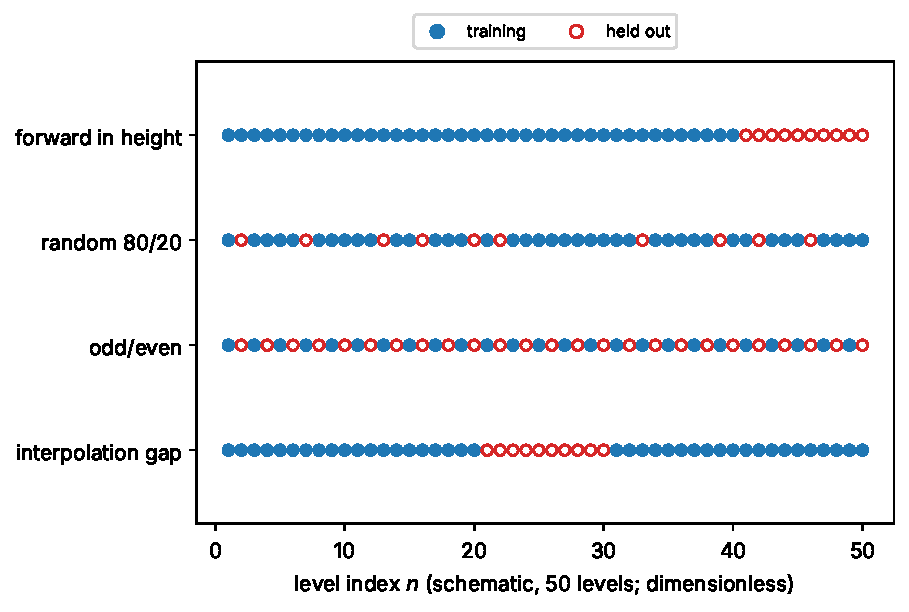
\includegraphics[width=0.85\linewidth]{figs/generalization_splits.pdf}
\caption{Schematic of four train/test splits on 50 level indices. Filled circles: training levels; open circles: held-out levels. Forward split: hold out the highest indices (extrapolation in height, with covariate shift). Random 80/20: hold out a random fifth (interpolation within one height range). Odd/even: train on odd indices, score on even (interpolation; every held-out level has training neighbors on both sides). Interpolation gap: hold out a contiguous interior block. The horizontal axis is the level index $n$ (dimensionless).}
\label{fig:generalization-splits}
\end{figure}

\begin{table}[htbp]\centering
\caption{Split types and what each tests. ``Paper'' gives where the split is used in the paper~\cite{soniR1}.}
\label{tab:generalization-splits}
\small
\begin{tabular}{llll}
\toprule
split & held-out levels & tests & paper \\
\midrule
forward & above training range & extrapolation in height & Tables I, II, IV, V \\
random 80/20 & random fifth, same range & interpolation, no height shift & Table III, Sec.~II~C \\
odd/even & alternate levels & interpolation from both neighbors & Table III \\
interpolation gap & interior block & interpolation over a gap & Sec.~III, Fig.~4 \\
\bottomrule
\end{tabular}
\end{table}

\begin{sample}{Counting levels and checking saturation in the within-height splits}
At scale 1 the paper's within-height splits are drawn inside zeros 1--400 (Sec.~II~C). (a) How many levels are trained and held out in a random 80/20 split? (b) In an odd/even split? (c) For which of the basis sizes $M=100,200,400$ is the odd/even fit at or above saturation?

Step 1: Random 80/20 of 400: held out $400/5=80$ (the paper draws them with \texttt{rng.choice(n, n/5, replace=False)}, App.~A step 17); trained $400-80=320$.

Step 2: Odd/even: the odd indices $1,3,\dots,399$ are $200$ levels; the even indices $2,4,\dots,400$ are another $200$. Each direction trains on 200 and scores 200.

Step 3: Saturation requires at least as many coefficients as training levels: $M\ge200$. So $M=200$ and $M=400$ are at or above the threshold; $M=100$ is below it.

\[
\boxed{\text{(a) }320/80;\quad\text{(b) }200/200;\quad\text{(c) }M=200,400}
\]
This is why the paper calls the odd/even rows with $M\ge200$ ``saturated'' and ``stress tests of memorization,'' and adds an $M=100$ row (Table~III).
\end{sample}

\begin{pitfall}
Each split has its own null. Because the held-out levels differ, the null rms differs too: in Table~III it is $0.238$ for the even-indexed held-out levels at scale 1 (``odd'' rows, trained on odd), $0.250$ for the odd-indexed ones, and $0.23$--$0.26$ across random seeds. Always compare a model's held-out error with the null \emph{on the same held-out set}.
\end{pitfall}

\begin{checkpoint}
A model fails a forward split (trained on 1--400, scored on 401--500) but succeeds on a random 80/20 split inside 1--400. Which explanation does this pattern support: covariate shift, or failure to capture structure?
\end{checkpoint}
\checkanswer{It points toward the forward failure being (at least partly) a problem of extrapolation or covariate shift, since the model does capture something usable within one height range. The reverse pattern (failure within height as well) rules covariate shift out as the explanation.}

\begin{keyideas}
\item Interpolation (test among training points) and extrapolation (test beyond them) can give opposite verdicts for the same fit.
\item Forward splits of the zeros involve a mild covariate shift: the null grows from $0.263$ (401--500) to $0.296$ (5001--10000).
\item Within-height splits (random, odd/even) remove the height shift; each split has its own null.
\end{keyideas}

%======================================================================
\section{Serial correlation: when smooth interpolation is anticorrelated with truth}\label{sec:generalization-serial}

\subsection{Stationary sequences and their autocorrelation}

A natural way to predict a held-out value in a sequence is to look at its neighbors. Whether that works depends on how neighbors are correlated.

Consider a sequence $d_1,d_2,\dots$ (for us, the fluctuations of Eq.~\eqref{eq:generalization-dn}). Treat it as random, and suppose it is \emph{stationary}: its statistics do not depend on the position $n$. Concretely we assume
\begin{equation}
\langle d_n\rangle=0,\qquad \langle d_n^2\rangle=\sigma^2,\qquad \langle d_nd_{n+k}\rangle=\sigma^2\rho_k,
\label{eq:generalization-stat}
\end{equation}
where $\langle\cdot\rangle$ denotes an average (expectation) and $\rho_k$ is the \emph{autocorrelation at lag $k$} (Chapter~\ref{ch:probability}); $\rho_0=1$ and $\rho_{-k}=\rho_k$. For the zeros, stationarity is an approximation that holds within a limited height range: the null rms drifts slowly (Sec.~\ref{sec:generalization-shift}), and we neglect that drift.

\subsection{The neighbor-mean predictor}

The simplest smooth interpolator predicts a held-out value as the average of its two neighbors:
\begin{equation}
\hat d_n=\tfrac12\bigl(d_{n-1}+d_{n+1}\bigr).
\label{eq:generalization-nbr}
\end{equation}
We compute its correlation with the truth and its mean squared error, using only Eq.~\eqref{eq:generalization-stat}.

\emph{Covariance with the truth:}
\begin{align}
\langle\hat d_nd_n\rangle&=\tfrac12\langle d_{n-1}d_n\rangle+\tfrac12\langle d_{n+1}d_n\rangle&&\text{(linearity of the average)}\notag\\
&=\tfrac12\sigma^2\rho_1+\tfrac12\sigma^2\rho_1&&\text{(both pairs are at lag 1)}\notag\\
&=\sigma^2\rho_1.
\end{align}
\emph{Variance of the prediction:}
\begin{align}
\langle\hat d_n^{\,2}\rangle&=\tfrac14\langle(d_{n-1}+d_{n+1})^2\rangle\notag\\
&=\tfrac14\bigl(\langle d_{n-1}^2\rangle+2\langle d_{n-1}d_{n+1}\rangle+\langle d_{n+1}^2\rangle\bigr)&&\text{(expand the square)}\notag\\
&=\tfrac14\bigl(\sigma^2+2\sigma^2\rho_2+\sigma^2\bigr)&&\text{($n-1$ and $n+1$ are at lag 2)}\notag\\
&=\tfrac12\sigma^2(1+\rho_2).
\end{align}
\emph{Correlation} (covariance divided by the product of standard deviations):
\begin{equation}
\mathrm{corr}(\hat d,d)=\frac{\sigma^2\rho_1}{\sigma\cdot\sigma\sqrt{(1+\rho_2)/2}}=\rho_1\sqrt{\frac{2}{1+\rho_2}}.
\label{eq:generalization-nbrcorr}
\end{equation}
\emph{Mean squared error:}
\begin{align}
\langle(\hat d_n-d_n)^2\rangle&=\langle\hat d_n^{\,2}\rangle-2\langle\hat d_nd_n\rangle+\langle d_n^2\rangle\notag\\
&=\sigma^2\left[\frac{1+\rho_2}{2}-2\rho_1+1\right].
\label{eq:generalization-nbrmse}
\end{align}

The conclusion is immediate from Eq.~\eqref{eq:generalization-nbrcorr}: since $\sqrt{2/(1+\rho_2)}>0$, \textbf{the neighbor mean has the sign of $\rho_1$}. If consecutive values are negatively correlated, interpolating between neighbors is anticorrelated with the truth, and by Eq.~\eqref{eq:generalization-nbrmse} its error exceeds the null's ($\sigma^2$) whenever $(1+\rho_2)/2-2\rho_1>0$, which certainly holds when $\rho_1<0$ (because $1+\rho_2\ge0$ for any valid autocorrelation).

The same holds for any interpolator that averages nearby neighbors with positive weights, $\hat d_n=\sum_{k\ge1}w_k(d_{n-k}+d_{n+k})$ with $w_k\ge0$: by the same steps, $\langle\hat d_nd_n\rangle=2\sigma^2\sum_kw_k\rho_k$, which is negative when the weights sit mostly on lags where $\rho_k<0$.

\begin{sample}{Anticorrelation by construction}
A stationary sequence has $\rho_1=-0.3$ and $\rho_2=-0.1$. Find the correlation of the neighbor-mean predictor with the truth and the ratio of its rms error to the null.

Step 1: Correlation from Eq.~\eqref{eq:generalization-nbrcorr}: $-0.3\sqrt{2/0.9}=-0.3\times1.4907=-0.447$.

Step 2: MSE from Eq.~\eqref{eq:generalization-nbrmse}: $\sigma^2[0.9/2+0.6+1]=2.05\,\sigma^2$.

Step 3: rms ratio: $\sqrt{2.05}=1.432$.

\[
\boxed{\mathrm{corr}=-0.447,\qquad \mathrm{rms}/\mathrm{rms}_{\rm null}=1.43}
\]
\end{sample}

\subsection{Why the zeros have negative lag-1 correlation}

Is $\rho_1<0$ plausible for the zeros? There is a simple approximate relation behind it. Define the unfolded spacing $u_n=(t_{n+1}-t_n)/\gap_n$. Using $t_n=s_n+\gap_n d_n$ and the approximation $s_{n+1}-s_n\approx\gap_n$, $\gap_{n+1}\approx\gap_n$ (the mean spacing changes slowly from one level to the next; we neglect its change),
\begin{equation}
u_n\approx\frac{s_{n+1}-s_n}{\gap_n}+d_{n+1}-d_n\approx1+d_{n+1}-d_n.
\label{eq:generalization-un}
\end{equation}
Then, using Eq.~\eqref{eq:generalization-stat},
\begin{align}
\mathrm{Var}(u)&=\langle(d_{n+1}-d_n)^2\rangle\notag\\
&=\langle d_{n+1}^2\rangle-2\langle d_{n+1}d_n\rangle+\langle d_n^2\rangle\notag\\
&=2\sigma^2(1-\rho_1),
\end{align}
and solving for $\rho_1$,
\begin{equation}
\rho_1=1-\frac{\mathrm{Var}(u)}{2\sigma^2}.
\label{eq:generalization-rho1}
\end{equation}
For a perfectly regular lattice with independent jitter of each level, $d_n$ independent gives $\rho_1=0$ and $\mathrm{Var}(u)=2\sigma^2$, consistent with Eq.~\eqref{eq:generalization-rho1}. Eq.~\eqref{eq:generalization-rho1} says when $\rho_1$ is negative: $\rho_1<0$ if and only if $\mathrm{Var}(u)>2\sigma^2$. The sign is therefore decided by comparing two numbers, the variance of the unfolded spacings and twice the variance of the fluctuations. For the zeros the next Sample Problem gives $\mathrm{Var}(u)\approx0.178$ (from the Wigner surmise, Chapter~\ref{ch:level-statistics}) against $2\sigma^2\approx0.138$ (from the measured null rms $0.263$), so the inequality holds and $\rho_1<0$. In words: the positions stay close to their smooth values (small $\sigma$, often called \emph{rigidity}), while consecutive spacings vary by more than independent jitter of that size would produce. The two facts are compatible only if neighboring zeros tend to be displaced in opposite directions (when one sits above its smooth position the next tends to sit below), which is what a negative $\rho_1$ means.

\begin{sample}{Estimating $\rho_1$ for the zeros from the Wigner surmise}
Estimate $\rho_1$ for the zero fluctuations using Eq.~\eqref{eq:generalization-rho1}, taking $\mathrm{Var}(u)$ from the GUE Wigner surmise $p(s)=\frac{32}{\pi^2}s^2e^{-4s^2/\pi}$ (paper Fig.~2; Chapter~\ref{ch:level-statistics}) and $\sigma=0.263$, the null rms on zeros 401--500.

Step 1: Recall from Chapter~\ref{ch:level-statistics} that the Wigner surmise $p(s)$ is an approximate probability density for the unfolded spacings: $\int_0^\infty p(s)\,ds=1$, and its mean is 1. We check the mean. Write $b=4/\pi$. Then $\langle s\rangle=\frac{32}{\pi^2}\int_0^\infty s^3e^{-bs^2}\,ds$. Substitute $u=s^2$, $du=2s\,ds$: $\int_0^\infty s^3e^{-bs^2}\,ds=\frac12\int_0^\infty u\,e^{-bu}\,du=\frac12\cdot\frac1{b^2}$ (integration by parts). With $b^2=16/\pi^2$ this is $\pi^2/32$, so $\langle s\rangle=\frac{32}{\pi^2}\cdot\frac{\pi^2}{32}=1$. Taking the spacings $u$ to follow the surmise, $\mathrm{Var}(u)=\langle s^2\rangle-\langle s\rangle^2=\langle s^2\rangle-1$, with $\langle s^2\rangle=\frac{32}{\pi^2}\int_0^\infty s^4e^{-bs^2}\,ds$.

Step 2: Start from the Gaussian integral $\int_0^\infty e^{-bs^2}ds=\frac12\sqrt{\pi}\,b^{-1/2}$ (Chapter~\ref{ch:probability}). Differentiating with respect to $b$ under the integral sign (a step we take on trust here; it is justified in~\cite{rhb}) brings down a factor $-s^2$ each time. Once:
\[
\int_0^\infty s^2e^{-bs^2}ds=-\frac{d}{db}\Bigl(\tfrac12\sqrt\pi\,b^{-1/2}\Bigr)=\tfrac14\sqrt\pi\,b^{-3/2}.
\]
Twice:
\[
\int_0^\infty s^4e^{-bs^2}ds=-\frac{d}{db}\Bigl(\tfrac14\sqrt\pi\,b^{-3/2}\Bigr)=\tfrac38\sqrt\pi\,b^{-5/2}.
\]
With $b^{-5/2}=(\pi/4)^{5/2}=\pi^{5/2}/32$:
\[
\langle s^2\rangle=\frac{32}{\pi^2}\cdot\frac38\sqrt\pi\cdot\frac{\pi^{5/2}}{32}=\frac{3\pi^3}{8\pi^2}=\frac{3\pi}{8}=1.1781.
\]
So $\mathrm{Var}(u)=0.1781$.

Step 3: $2\sigma^2=2(0.263)^2=0.1383$.

Step 4: $\rho_1\approx1-0.1781/0.1383=1-1.287=-0.287$.

\[
\boxed{\rho_1\approx-0.29}
\]
This is an estimate, not a measurement: the surmise is an approximation to the true spacing law, Eq.~\eqref{eq:generalization-un} neglects the slow change of $\gap_n$, and stationarity is approximate. It does show that negative $\rho_1$ is the expected sign. How large is the measured value? The paper's measured correlations of the mean of the two nearest training fluctuations with the truth are $-0.26$ to $-0.41$ (Sec.~III). Inverting Eq.~\eqref{eq:generalization-nbrcorr} with $\rho_2=0$ gives $\rho_1=\mathrm{corr}/\sqrt2$, between about $-0.18$ and $-0.29$; a negative $\rho_2$, which the paper also reports, would make $\abs{\rho_1}$ somewhat smaller. (This inversion is approximate: in the random splits the nearest training neighbors are not always at lag 1.) So the estimate $-0.29$ has the right sign and the right size, at the large end of the range. You can measure $\rho_1$ directly with the listing below (Problem~8). The paper reports that ``the fluctuation sequence has negative autocorrelation at lags 1--3'' (Sec.~III).
\end{sample}

Figure~\ref{fig:generalization-neighbor} shows the real fluctuations of zeros 1--400 computed with \texttt{qmnt}, the neighbor-mean prediction for the even-indexed levels from their odd neighbors, and the sample autocorrelation. When you run the listing below, you will find that the measured lag-1 autocorrelation of zeros 1--400 is negative, that the neighbor-mean prediction for the even-indexed levels is anticorrelated with the truth, and that its rms error is above the null of those levels, as Eqs.~\eqref{eq:generalization-nbrcorr} and~\eqref{eq:generalization-nbrmse} predict for $\rho_1<0$.

\begin{figure}[htbp]\centering
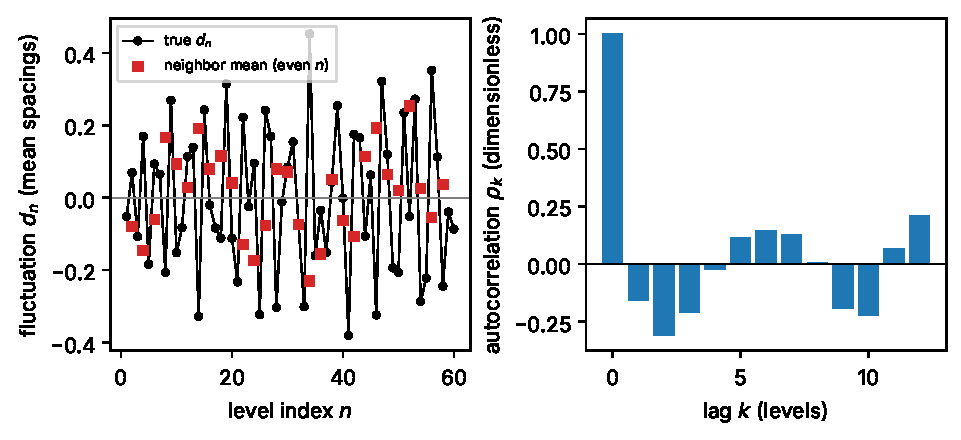
\includegraphics[width=0.95\linewidth]{figs/generalization_neighbor.pdf}
\caption{Left: fluctuations $d_n=(t_n-s_n)/\gap_n$ of zeros 1--60 (black, in mean spacings) and the neighbor-mean prediction $\tfrac12(d_{n-1}+d_{n+1})$ for even $n$ (red squares). Where $d_n$ is high its neighbors tend to be low, so the prediction tends to have the wrong sign. Right: sample autocorrelation $\rho_k$ of $d_n$ for zeros 1--400 against lag $k$ (in levels); the lag-1 value is negative (the paper reports negative values at lags 1--3, Sec.~III).}
\label{fig:generalization-neighbor}
\end{figure}

\begin{pycode}
import numpy as np, qmnt
t = qmnt.zeros(400); n = np.arange(1, 401)
d = qmnt.fluct(t, n)
dc = d - d.mean()
for k in range(1, 6):
    print("lag", k, np.sum(dc[:-k] * dc[k:]) / np.sum(dc**2))
ev = np.arange(1, 399, 2)               # positions of n = 2, 4, ..., 398
pred = 0.5 * (d[ev - 1] + d[ev + 1])    # mean of the two odd neighbors
print("neighbor mean: rms", qmnt.rms(pred - d[ev]), "corr", qmnt.corr(pred, d[ev]))
print("null rms", qmnt.rms(d[ev]))
\end{pycode}

\begin{checkpoint}
If a sequence had $\rho_1=+0.8$, would the neighbor-mean predictor be correlated or anticorrelated with the truth?
\end{checkpoint}
\checkanswer{Positively correlated: by Eq.~\eqref{eq:generalization-nbrcorr} the correlation has the sign of $\rho_1$.}

\begin{keyideas}
\item For a stationary sequence, the neighbor mean has correlation $\rho_1\sqrt{2/(1+\rho_2)}$ with the truth: its sign is the sign of $\rho_1$.
\item The identity $\rho_1=1-\mathrm{Var}(u)/(2\sigma^2)$ links lag-1 correlation to spacing variance and position rigidity; for the zeros it predicts $\rho_1<0$ (estimate $\approx-0.29$).
\item Hence any interpolator that averages nearby neighboring zeros with positive weights tends to be anticorrelated with the truth; a correlation-aware predictor (Sec.~\ref{sec:generalization-kriging}) need not be.
\end{keyideas}

%======================================================================
\section{The best linear predictor: simple kriging}\label{sec:generalization-kriging}

\subsection{Deriving the normal equations}

If neighbor averaging has the wrong sign, what is the \emph{right} way to use neighbors? Ask for the linear combination of training values that minimizes the expected squared error. This is called the \emph{best linear predictor}, or \emph{simple kriging} (a name from geostatistics, where it was developed to interpolate ore grades between boreholes; ``simple'' means the mean is known, here zero).

Let the value to predict be $d_0$ and the available training values be $d_1,\dots,d_K$ (any positions). Write $C_{ij}=\langle d_id_j\rangle$ for their covariances, collected in the $K\times K$ matrix $C$, and $\bm c_0$ for the vector with entries $C_{i0}=\langle d_id_0\rangle$. (In this section only, $\bm c_0$ is this covariance vector, not a coefficient of $\delta V$.) The predictor is $\hat d_0=\sum_{i=1}^Kw_id_i=\bm w^\top\bm d$. Its mean squared error is
\begin{align}
\mathcal E(\bm w)&=\Bigl\langle\Bigl(d_0-\sum_iw_id_i\Bigr)^2\Bigr\rangle\notag\\
&=\langle d_0^2\rangle-2\sum_iw_i\langle d_id_0\rangle+\sum_i\sum_jw_iw_j\langle d_id_j\rangle&&\text{(expand the square)}\notag\\
&=C_{00}-2\sum_iw_iC_{i0}+\sum_i\sum_jw_iw_jC_{ij}.
\label{eq:generalization-krigE}
\end{align}
Differentiate with respect to one weight $w_k$, holding all the other weights fixed (a partial derivative: ordinary differentiation in which the other weights are treated as constants). The middle term gives $-2C_{k0}$. In the double sum, $w_k$ appears when $i=k$ (giving $\sum_jw_jC_{kj}$) and when $j=k$ (giving $\sum_iw_iC_{ik}$); since $C_{ik}=C_{ki}$ these are equal, totalling $2\sum_jC_{kj}w_j$. Setting the derivative to zero:
\begin{equation}
-2C_{k0}+2\sum_jC_{kj}w_j=0\quad\Longrightarrow\quad\sum_{j=1}^KC_{kj}w_j=C_{k0},\quad k=1,\dots,K,
\end{equation}
or in matrix form
\begin{equation}
C\bm w=\bm c_0.
\label{eq:generalization-krig}
\end{equation}
These are the \emph{kriging normal equations}. They have the same structure as the least-squares normal equations of Chapter~\ref{ch:least-squares}, with covariances in place of sums of products. To see that the solution is a minimum and not some other stationary point, change the weights from $\bm w$ to $\bm w+\bm v$ for an arbitrary vector $\bm v$. From Eq.~\eqref{eq:generalization-krigE} in matrix form, $\mathcal E(\bm w)=C_{00}-2\bm w^\top\bm c_0+\bm w^\top C\bm w$, so
\begin{align}
\mathcal E(\bm w+\bm v)&=C_{00}-2(\bm w+\bm v)^\top\bm c_0+(\bm w+\bm v)^\top C(\bm w+\bm v)\notag\\
&=\mathcal E(\bm w)-2\bm v^\top\bm c_0+2\bm v^\top C\bm w+\bm v^\top C\bm v&&\text{($C$ symmetric, so $\bm w^\top C\bm v=\bm v^\top C\bm w$)}\notag\\
&=\mathcal E(\bm w)+2\bm v^\top(C\bm w-\bm c_0)+\bm v^\top C\bm v.\notag
\end{align}
If $\bm w$ solves $C\bm w=\bm c_0$, the middle term vanishes, and $\bm v^\top C\bm v=\sum_i\sum_jv_iv_j\langle d_id_j\rangle=\langle(\bm v^\top\bm d)^2\rangle\ge0$. Hence $\mathcal E(\bm w+\bm v)\ge\mathcal E(\bm w)$ for every $\bm v$: the solution is a minimum.

\emph{Minimum error.} At the solution, $\bm w^\top C\bm w=\bm w^\top\bm c_0$ (multiply Eq.~\eqref{eq:generalization-krig} by $\bm w^\top$), so Eq.~\eqref{eq:generalization-krigE} becomes
\begin{equation}
\mathcal E_{\min}=C_{00}-2\bm w^\top\bm c_0+\bm w^\top\bm c_0=C_{00}-\bm w^\top\bm c_0.
\label{eq:generalization-krigmin}
\end{equation}

\emph{Orthogonality.} The normal equations say $\langle(d_0-\hat d_0)d_k\rangle=C_{k0}-\sum_jw_jC_{kj}=0$ for every $k$: the error of the best linear predictor is uncorrelated with every piece of data it used. If it were not, some multiple of that piece could be added to reduce the error further.

\subsection{Two neighbors: the sign flips}

Predict $d_n$ from $d_{n-1}$ and $d_{n+1}$. With Eq.~\eqref{eq:generalization-stat}, $C=\sigma^2\begin{pmatrix}1&\rho_2\\\rho_2&1\end{pmatrix}$ and $\bm c_0=\sigma^2\begin{pmatrix}\rho_1\\\rho_1\end{pmatrix}$. The equations are $w_1+\rho_2w_2=\rho_1$ and $\rho_2w_1+w_2=\rho_1$. Subtracting the second from the first gives $(1-\rho_2)(w_1-w_2)=0$, so $w_1=w_2\equiv w$ (provided $\rho_2\ne1$). Then $w(1+\rho_2)=\rho_1$:
\begin{equation}
w=\frac{\rho_1}{1+\rho_2},\qquad \hat d_n=w\,(d_{n-1}+d_{n+1}).
\label{eq:generalization-w}
\end{equation}
From Eq.~\eqref{eq:generalization-krigmin}, $\mathcal E_{\min}=\sigma^2-2w\sigma^2\rho_1=\sigma^2\Bigl(1-\dfrac{2\rho_1^2}{1+\rho_2}\Bigr)$, which is never larger than the null $\sigma^2$.

Now compare with the neighbor mean. The kriging predictor is $\hat d_n=2w\times\tfrac12(d_{n-1}+d_{n+1})$, a constant multiple of the neighbor mean. Multiplying a variable by a constant $\alpha\ne0$ multiplies its correlation with anything by the sign of $\alpha$. To see this, recall from Chapter~\ref{ch:probability} that $\mathrm{Cov}(\alpha X,Y)=\alpha\,\mathrm{Cov}(X,Y)$ and that the standard deviation of $\alpha X$ is $\abs{\alpha}$ times that of $X$. Then
\[
\mathrm{corr}(\alpha X,Y)=\frac{\alpha\,\mathrm{Cov}(X,Y)}{\abs{\alpha}\,\mathrm{sd}(X)\,\mathrm{sd}(Y)}=\frac{\alpha}{\abs{\alpha}}\,\mathrm{corr}(X,Y)=\mathrm{sign}(\alpha)\,\mathrm{corr}(X,Y).
\]
The magnitude of the correlation is unchanged; only its sign can change. Here $\alpha=2w$. When $\rho_1<0$ we have $w<0$, so

\medskip\noindent\textbf{Result (proved).} When $w<0$, the two-neighbor kriging prediction and the neighbor mean have correlations with the truth that are equal in magnitude and opposite in sign. With $\rho_1<0$ the neighbor mean is anticorrelated and kriging is positively correlated, $\mathrm{corr}=\abs{\rho_1}\sqrt{2/(1+\rho_2)}$.

\medskip
The best linear use of negatively correlated neighbors is to predict the \emph{opposite} of their average, shrunk toward zero.

\begin{sample}{Kriging versus the neighbor mean}
Use $\rho_1=-0.3$, $\rho_2=-0.1$ as in the earlier Sample Problem ``Anticorrelation by construction''. Find the kriging weight, the error ratio and the correlation, and compare.

Step 1: $w=-0.3/(1-0.1)=-0.3/0.9=-0.3333$.

Step 2: $\mathcal E_{\min}/\sigma^2=1-2(0.09)/0.9=1-0.2=0.8$; rms ratio $\sqrt{0.8}=0.894$.

Step 3: Correlation. $\mathrm{Var}(\hat d)=w^2\cdot2\sigma^2(1+\rho_2)=\frac19\cdot2(0.9)\sigma^2=0.2\sigma^2$ and $\langle\hat dd\rangle=2w\sigma^2\rho_1=2(-\tfrac13)(-0.3)\sigma^2=0.2\sigma^2$. So $\mathrm{corr}=0.2\sigma^2/(\sigma\sqrt{0.2}\,\sigma)=\sqrt{0.2}=0.447$.

\[
\boxed{w=-\tfrac13,\quad \mathrm{rms}/\mathrm{rms}_{\rm null}=0.894,\quad \mathrm{corr}=+0.447\ (\text{neighbor mean: }-0.447,\ 1.43)}
\]
Note that $\mathrm{corr}^2=0.2=1-\mathcal E_{\min}/\sigma^2$, which agrees with the optimum $\sqrt{1-\rho^2}$ of Eq.~\eqref{eq:generalization-ratio}: kriging automatically chooses the best amplitude.
\end{sample}

\begin{figure}[htbp]\centering
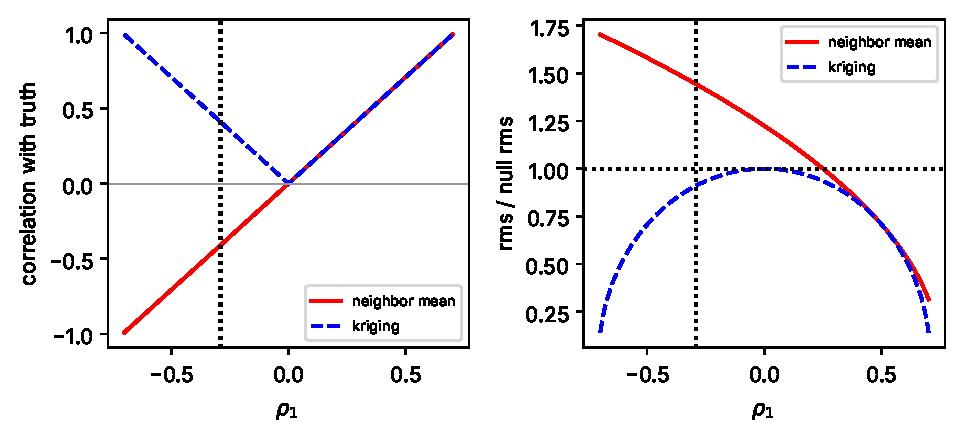
\includegraphics[width=0.95\linewidth]{figs/generalization_kriging.pdf}
\caption{Neighbor mean versus two-neighbor kriging for a stationary sequence with lag-2 correlation $\rho_2=0$, as functions of the lag-1 correlation $\rho_1$ (dimensionless). Left: correlation with the truth, Eq.~\eqref{eq:generalization-nbrcorr} and its kriging counterpart. Right: rms error relative to the null (dotted line at 1). The vertical dotted line marks the estimate $\rho_1\approx-0.29$ for the zeros from the Sample Problem on the Wigner surmise. For $\rho_1<0$ the neighbor mean is anticorrelated and worse than the null; kriging is positively correlated and better than the null. The plotted range is $\abs{\rho_1}\le1/\sqrt2$: with $\rho_2=0$ the neighbor-mean correlation is $\sqrt2\,\rho_1$, which must lie in $[-1,1]$; equivalently, the correlation matrix of $(d_{n-1},d_n,d_{n+1})$, whose determinant is $1-2\rho_1^2$, is a valid covariance only if $1-2\rho_1^2\ge0$.}
\label{fig:generalization-kriging}
\end{figure}

\subsection{The nugget}

In practice the covariances are estimated from data, and the estimated $C$ may be nearly singular or even slightly inconsistent. Geostatisticians add a \emph{nugget}: a constant $\tau^2$ on the diagonal,
\begin{equation}
(C+\tau^2I)\,\bm w=\bm c_0.
\label{eq:generalization-nugget}
\end{equation}
There are two ways to read it. (i) If each observed training value carries independent measurement noise of variance $\tau^2$, the covariances among the \emph{observations} are $C_{ij}+\tau^2\delta_{ij}$ (where $\delta_{ij}=1$ if $i=j$ and $0$ otherwise), while their covariances with the noiseless target are unchanged; Eq.~\eqref{eq:generalization-nugget} is then the exact best predictor. (ii) As a regularizer, it is the kriging cousin of ridge regression (Chapter~\ref{ch:least-squares}): a larger nugget shrinks $\bm w$ toward zero and the prediction toward the null. In the two-neighbor case the weight becomes $w=\rho_1/(1+\rho_2+\tau^2/\sigma^2)$.

\begin{sample}{The price of a small nugget}
With $\rho_1=-0.3$, $\rho_2=-0.1$, add a nugget $\tau^2/\sigma^2=0.05$ as a pure regularizer (the data themselves are noiseless). Find $w$ and the true MSE.

Step 1: $w=-0.3/(0.9+0.05)=-0.3158$.

Step 2: For noiseless data, Eq.~\eqref{eq:generalization-krigE} with two equal weights gives $\mathcal E/\sigma^2=1-4w\rho_1+2w^2(1+\rho_2)$.

Step 3: $-4w\rho_1=-4(-0.3158)(-0.3)=-0.3789$ and $2w^2(0.9)=2(0.09972)(0.9)=0.1795$, so $\mathcal E/\sigma^2=1-0.3789+0.1795=0.8006$.

\[
\boxed{w=-0.316,\qquad \mathcal E/\sigma^2=0.8006\ \ (\text{optimum }0.8)}
\]
A small nugget costs almost nothing in accuracy and buys numerical stability. The paper's kriging used a nugget of $0.05$, added once ``after a first version without them was numerically unstable, and not tuned'' (App.~A step 19).
\end{sample}

Now try two-neighbor kriging on the real zeros. The listing below makes a random 80/20 split of zeros 1--400 (seed 1), estimates $\rho_1$ and $\rho_2$ from pairs of training levels only, and predicts every held-out level whose two neighbors are both training levels, first by the neighbor mean and then by Eq.~\eqref{eq:generalization-w}. It subtracts the training mean first, because the sample mean of the fluctuations is not exactly zero. (In the listing the variable \texttt{mu} is that mean, not a ridge strength.)

\begin{pycode}
import numpy as np, qmnt
t = qmnt.zeros(400); n = np.arange(1, 401); d = qmnt.fluct(t, n)
rng = np.random.default_rng(1)
test = np.zeros(400, bool); test[rng.choice(400, 80, replace=False)] = True
train = ~test
mu = d[train].mean()
def acf(k):                         # autocorrelation from training pairs only
    i = np.arange(400 - k)
    ok = train[i] & train[i + k]
    a, b = d[i[ok]] - mu, d[i[ok] + k] - mu
    return np.mean(a * b) / np.var(d[train])
r1, r2 = acf(1), acf(2)
w = r1 / (1 + r2)
# held-out levels whose two neighbors are both training levels
j = np.array([i for i in range(1, 399) if test[i] and train[i-1] and train[i+1]])
s = (d[j-1] - mu) + (d[j+1] - mu)
for name, pred in [("neighbor mean", mu + 0.5*s), ("kriging", mu + w*s)]:
    print(name, qmnt.rms(pred - d[j]), qmnt.corr(pred, d[j]))
print("null", qmnt.rms(d[j]))
\end{pycode}

When you run it, the estimated weight $w$ comes out negative, the neighbor mean is anticorrelated with the held-out truth, and the kriging prediction is positively correlated with it, with exactly the same magnitude of correlation, as the Result above requires. Compare the two printed rms values with the printed null yourself.

\begin{pitfall}
Estimating correlations with the test data. In the listing above the autocorrelations come only from pairs of \emph{training} levels. In an odd/even split this matters sharply: no two training levels are adjacent, so $\rho_1$ cannot be estimated from the training set at all. Using all levels to estimate $\rho_1$ would leak held-out information into the predictor.
\end{pitfall}

\begin{beyond}
For a sequence whose joint distribution is Gaussian (a ``Gaussian process''), the best linear predictor is also the best predictor of \emph{any} form, linear or not: the conditional mean of $d_0$ given the data is exactly $\bm w^\top\bm d$ with $\bm w$ from Eq.~\eqref{eq:generalization-krig}. We do not use this; it is proved in standard texts on multivariate statistics and Gaussian processes. Everything in this section is proved for linear predictors only.
\end{beyond}

\begin{keyideas}
\item The best linear predictor solves the kriging normal equations $C\bm w=\bm c_0$; its error is uncorrelated with the data used.
\item With two neighbors, $w=\rho_1/(1+\rho_2)$; for $\rho_1<0$ the prediction is a negative, shrunken multiple of the neighbor sum, and its correlation equals that of the neighbor mean with the sign flipped.
\item A nugget $(C+\tau^2I)\bm w=\bm c_0$ stabilizes the solve and shrinks toward the null, like ridge.
\end{keyideas}

%======================================================================
\section{Regularization: the road back to the null}\label{sec:generalization-ridge}
% DYK-BEGIN
\begin{didyouknow}{Fitting an Elephant}
Freeman Dyson recalled that in 1953 Enrico Fermi dismissed a complicated model by quoting John von Neumann: \emph{with four parameters I can fit an elephant, and with five I can make him wiggle his trunk}. In 2010 three physicists actually drew an elephant using four complex parameters. Regularization is the disciplined way to stop extra parameters from fitting elephants.
\end{didyouknow}
% DYK-END

\subsection{Ridge in one parameter}

Recall ridge (Tikhonov) regularization from Chapter~\ref{ch:least-squares}. We write it in the paper's convention: minimize $\norm{X\bm c-\bm y}^2+\mu\sigma_1^2\norm{\bm c}^2$, where $\sigma_1$ is the largest singular value of the design matrix $X$. The penalty punishes large coefficients; scaling it by $\sigma_1^2$ makes $\mu$ a pure number that measures the penalty relative to the most strongly determined direction of the data. In the simplest case, a single parameter $c$ and the model $f(x)=cx$, the design matrix is the single column $(x_1,\dots,x_n)^\top$, and its only singular value is the length of that column, $\sigma_1=(\sum_ix_i^2)^{1/2}$ (Chapter~\ref{ch:least-squares}). The penalized error is therefore $S(c)=\sum_i(cx_i-y_i)^2+\mu\bigl(\sum_jx_j^2\bigr)c^2$. Setting $dS/dc=2\sum_ix_i(cx_i-y_i)+2\mu\bigl(\sum_jx_j^2\bigr)c=0$ gives $c\,(1+\mu)\sum_ix_i^2=\sum_ix_iy_i$, that is
\begin{equation}
c(\mu)=\frac{\sum_ix_iy_i}{(1+\mu)\sum_ix_i^2}.
\label{eq:generalization-ridge1}
\end{equation}
At $\mu=0$ this is ordinary least squares; as $\mu\to\infty$, $c(\mu)\to0$ and every prediction $c(\mu)x$ tends to zero. If ``zero'' is the null (no fluctuation), then \emph{strong regularization returns any model to the null}.

\begin{sample}{A ridge path}
Data: $(x,y)=(1,2.1),(2,3.9),(3,6.2)$. Fit $f=cx$ with ridge strengths $\mu=0$, $1$ and $10$ (in the convention of Eq.~\eqref{eq:generalization-ridge1}); give $c$, the in-sample rms for $\mu=0$ and $\mu=1$, and the prediction at $x=4$.

Step 1: $\sum x_iy_i=2.1+7.8+18.6=28.5$; $\sum x_i^2=1+4+9=14$.

Step 2: $c(0)=28.5/14=2.0357$; $c(1)=28.5/(2\times14)=28.5/28=1.0179$; $c(10)=28.5/(11\times14)=28.5/154=0.1851$.

Step 3: In-sample residuals at $\mu=0$: $2.1-2.0357=0.0643$, $3.9-4.0714=-0.1714$, $6.2-6.1071=0.0929$; rms $=\sqrt{(0.00413+0.02939+0.00862)/3}=0.119$. At $\mu=1$: residuals $1.0821$, $1.8643$, $3.1464$; rms $=\sqrt{(1.1710+3.4756+9.9000)/3}=2.20$.

Step 4: Predictions at $x=4$: $8.143$, $4.071$, $0.740$.

\[
\boxed{c=2.036,\ 1.018,\ 0.185;\quad E_{\rm in}(0)=0.119,\ E_{\rm in}(1)=2.20;\quad f(4)=8.14,\ 4.07,\ 0.74}
\]
In-sample error rises with $\mu$, and the prediction slides toward zero.
\end{sample}

\subsection{Ridge with many parameters}

Recall the SVD solution with filter factors from Chapter~\ref{ch:least-squares}: writing $X=U\Sigma V^\top$ with singular values $\sigma_1\ge\sigma_2\ge\dots$, the one-shot ridge solution in the convention above has the form
\begin{equation}
\bm c=V\,\mathrm{diag}\!\left(\frac{\sigma_j}{\sigma_j^2+\mu\sigma_1^2}\right)U^\top\bm y.
\label{eq:generalization-filter}
\end{equation}
This is the one-shot, linear analogue of what the paper does. The paper's fit of the potential is iterative (App.~A step 6): at each iteration it recomputes the sensitivity matrix, takes its SVD $U\Sigma V^\top$, and updates
\[
\bm c\;\leftarrow\;\bm c+V\,\mathrm{diag}\!\left(\frac{\sigma_j}{\sigma_j^2+(\lambda+\mu)\sigma_1^2}\right)U^\top\bm r,
\]
where $\bm r$ is the current residual vector and $\lambda$ the Levenberg--Marquardt damping (Chapter~\ref{ch:fitting}). The paper's ridge variant ``adds $\mu\Sigma_1^2$ to the filter denominator'' alongside $\lambda\Sigma_1^2$; it does not replace $\lambda$. Its $\mu$ is in the same $\sigma_1^2$-scaled convention as ours. Each filter factor satisfies $0\le\sigma_j/(\sigma_j^2+\mu\sigma_1^2)\le\sigma_j/(\mu\sigma_1^2)$, which tends to zero as $\mu\to\infty$. In the one-shot form every component of $\bm c$ therefore tends to zero. In the iterated form the same bound (with $\lambda+\mu$ in place of $\mu$) makes every step tend to zero, so $\bm c$ stays at its starting value $\bm c=\bm 0$. Either way $\delta V\to0$, and the predicted levels tend to the unperturbed (null) levels. For moderate $\mu$, the factor is suppressed most for small $\sigma_j$, i.e.\ for the parameter directions that the training data constrain least. Those are exactly the directions that, by the Result of Sec.~\ref{sec:generalization-overfit}, can produce arbitrary held-out behavior.

Figure~\ref{fig:generalization-ridge} shows this for RE4.

\begin{figure}[htbp]\centering
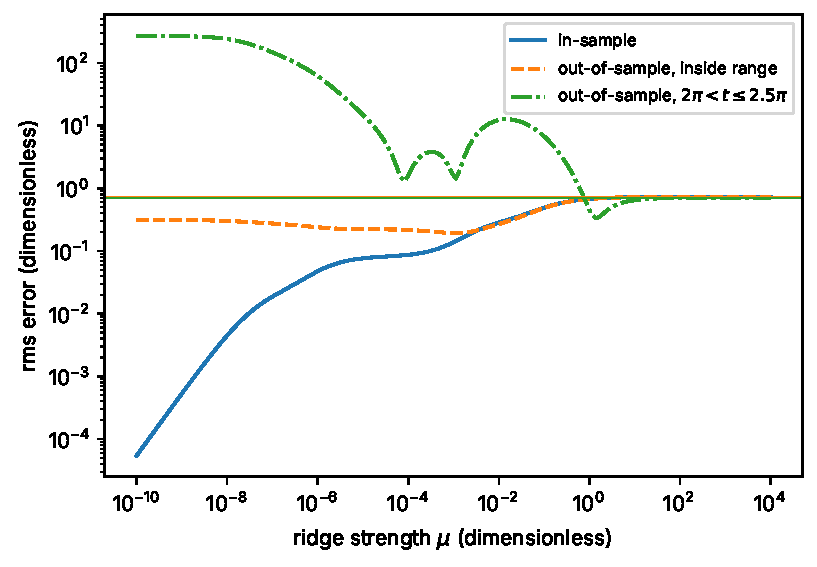
\includegraphics[width=0.85\linewidth]{figs/generalization_ridge.pdf}
\caption{Ridge path for RE4: a degree-9 polynomial (10 coefficients) fitted to 10 noisy samples of $\sin t$ on $0\le t\le2\pi$ with the filter of Eq.~\eqref{eq:generalization-filter}, as a function of the ridge strength $\mu$ (dimensionless, logarithmic). Solid: in-sample rms; dashed: out-of-sample rms inside the training range; dash-dotted: out-of-sample rms on $2\pi<t\le2.5\pi$. Thin horizontal lines: the corresponding nulls (rms of the test targets, i.e.\ the error of predicting zero). As $\mu$ grows every curve approaches its null.}
\label{fig:generalization-ridge}
\end{figure}

\begin{pitfall}
Believing ``regularization creates skill.'' Regularization can only \emph{select} among the behaviors the model already offers. If the family has the right structure (a good inductive bias), ridge helps by suppressing noise: the paper's control B, with arithmetic frequencies given and amplitudes fitted with ridge, predicts well (Table~IV; Chapter~\ref{ch:sparse-frequency}). If the family has no useful structure, ridge can only move it from ``memorize more'' toward ``do nothing.'' For the fitted potentials that is what the paper observed (Sec.~III); it is an empirical finding about those families, not a theorem about ridge.
\end{pitfall}

\begin{checkpoint}
As $\mu\to\infty$ in Eq.~\eqref{eq:generalization-filter}, what held-out rms does a ridge-fitted potential approach?
\end{checkpoint}
\checkanswer{The null rms, the error of the unperturbed potential's levels (for example $0.263$ on zeros 401--500), because $\bm c\to0$.}

\begin{keyideas}
\item Ridge shrinks coefficients; as $\mu\to\infty$ the fit tends to the null.
\item The filter $\sigma_j/(\sigma_j^2+\mu\sigma_1^2)$ suppresses poorly constrained directions first.
\item Regularization helps a model with a good inductive bias; it cannot supply a bias the model lacks.
\end{keyideas}

%======================================================================
\section{Inductive bias: a model that can fit anything}\label{sec:generalization-bias}

\subsection{Definition}

\textbf{Definition.} The \emph{inductive bias} of a fitting procedure is everything, apart from the training data, that determines its predictions on new inputs: the choice of model family, the basis, the starting point, the optimizer, the regularizer, the stopping rule.

Some bias is unavoidable. Two training points do not determine a value at a third point (Sample Problem ``Infinitely many perfect fits''); some rule must break the tie. ``Fit a straight line'' is a bias toward linear behavior; ``minimize the norm'' is a bias toward small coefficients; ``a few sinusoids'' is a bias toward sparsity in frequency. A procedure generalizes when its bias matches the process that generated the data.

\subsection{Why fitting anything means predicting nothing}

Combine the Result of Sec.~\ref{sec:generalization-overfit} with this definition. If a model family can fit \emph{any} training targets, and its training and test rows are jointly of full rank, then the set of perfect fits contains every possible held-out prediction. The data then carry no information about which prediction to make; the choice is made entirely by the bias. Unless that bias happens to match the truth, the predictions are, from the data's point of view, arbitrary. A family that can fit anything encodes no preference for the truth over any of its other perfect fits.

A sharp test follows. If a model fits \emph{scrambled} versions of the data (randomly permuted, or with randomized Fourier phases, Chapter~\ref{ch:fourier-transform}) as well as it fits the real data, then its in-sample accuracy measures its capacity, not anything specific to the real data. Chapter~\ref{ch:controls} develops these surrogate tests.

\begin{beyond}
In machine learning there are general ``no free lunch'' theorems, stating roughly that averaged over all possible target functions, no learning procedure outperforms any other on unseen inputs; any advantage comes from matching assumptions to the problem. We do not need or prove the general versions; the elementary linear Result of Sec.~\ref{sec:generalization-overfit} is the precise form we use. A textbook discussion of the role of model assumptions in prediction is~\cite{esl}.
\end{beyond}

\subsection{The fitted potential through this lens}

For the fitted potential, recall the first-order relation $\delta E_n\approx\sum_kA_{nk}c_k$ (Chapters~\ref{ch:perturbation} and~\ref{ch:fitting}). The levels feel the correction $\delta V$ through $|\psi_n|^2$, and recall from Chapter~\ref{ch:wkb} that a level of energy $E$ has \emph{classical turning points} at the positions where $V(x)=E$, where a classical particle of that energy would stop and reverse. The particle moves slowest there, and correspondingly $|\psi_n|^2$ is largest near the turning points, so a high level is most sensitive to $\delta V$ near them. A cosine correction with many terms can therefore shift the levels in almost any joint pattern, provided its basis is rich enough to resolve the local wavelength at the relevant energies. Chapter~\ref{ch:fitting} expressed this as the (heuristic) coverage law $M\pi/L>2\sqrt E$.

\begin{sample}{When is the cosine family complete for the scored levels?}
At scale 1 the box half-width is $L=44.883$ and the highest scored level sits near $E\approx t_{500}=811.184$ (paper App.~A key anchors). Use the coverage law to estimate the basis size $M$ beyond which the cosine family can realize essentially arbitrary shifts of all 500 levels. Compare $M=300$ and $M=900$.

Step 1: Solve $M\pi/L>2\sqrt E$ for $M$: $M>2\sqrt E\,L/\pi$.

Step 2: $\sqrt{811.184}=28.481$, so $2\sqrt E=56.963$.

Step 3: $M>56.963\times44.883/\pi=2556.7/\pi=813.8$.

Step 4: For $M=300$: $M\pi/L=300\pi/44.883=21.0<56.96$, not covered. For $M=900$: $900\pi/44.883=63.0>56.96$, covered.

\[
\boxed{M\gtrsim814}
\]
The paper reports in-sample rms $0.186$ on all 500 zeros at $M=300$ and below $10^{-4}$ at $M=900$, ``consistent with a basis-coverage law'' (Sec.~III). The law is a heuristic estimate, not a sharp threshold.
\end{sample}

How far does the Result of Sec.~\ref{sec:generalization-overfit} carry over? Its hypothesis is that the stacked training-plus-test matrix has full row rank. That requires $M\ge n_{\rm tr}+n_{\rm te}$; saturation on the training levels alone is not enough. Some of the paper's configurations meet the counting condition: $M=600$ fitted on zeros 1--400 and scored on 401--500 (500 rows, 600 columns), and the $M=400$ odd/even splits (400 rows). For these, provided the joint (linearized) sensitivity matrix has full row rank, exact training fits exist with any held-out shifts, and the data cannot choose among them. For the principal configuration, $M=400$ fitted on 400 zeros and scored on 100, the stacked matrix has 500 rows but rank at most 400, so the Result does not apply. There the held-out shifts are not completely free. They are only partly constrained, because parameter directions with small singular values of the training sensitivity matrix are weakly determined by the training levels, and such directions can move the held-out levels at little in-sample cost. In both cases, what the fitted potential predicts for the held-out levels is largely set by the optimizer: starting from $\bm c=\bm 0$, damped least-squares steps of the kind in Eq.~\eqref{eq:generalization-filter} build $\bm c$ from combinations of the rows of the training sensitivity matrix, and the held-out shifts are whatever those combinations happen to do to the held-out levels. This is a first-order, heuristic picture of a nonlinear fit; it explains the observed behavior without proving it.

\subsection{The right parametrization}

The explicit formula of Chapter~\ref{ch:explicit-formula} tells us what the fluctuations look like as functions of height $t$: a sum of sinusoids $\sin(mt\log p)$, an almost-periodic function (Chapter~\ref{ch:fourier-series}) that is \emph{sparse in frequency}. A bias toward ``a few sinusoids in $t$'' matches that structure, and a model with only that bias, and no knowledge of primes, can learn the frequencies from the zeros (Chapter~\ref{ch:sparse-frequency}). A cosine expansion of $\delta V(x)$ in position addresses each level locally through its turning points. Nothing in it says ``the pattern you saw at levels 1--400 continues at 401--500.'' The paper offers exactly this as a heuristic reading of its results (Sec.~VI); in Sec.~\ref{sec:generalization-paper} we see the experiment that isolates it.

\begin{checkpoint}
Two models fit the same 400 zeros to the same in-sample rms. Model P is a 400-coefficient potential; model S is a sum of 24 sinusoids in $t$ with fitted frequencies and amplitudes (72 parameters). Without looking at held-out data, can you say which will predict better?
\end{checkpoint}
\checkanswer{Not from the in-sample numbers alone; equal in-sample error says nothing about generalization. You can argue which inductive bias better matches the explicit formula (S), but the claim must be settled by held-out scores against the null.}

\begin{keyideas}
\item Inductive bias is everything besides the data that determines predictions on new inputs.
\item A family that can fit anything (including scrambled data) has its held-out predictions set largely by its bias, not by its data; fully so when training and test rows are jointly of full row rank ($M\ge n_{\rm tr}+n_{\rm te}$).
\item The coverage law estimates when the cosine family becomes effectively complete: $M\gtrsim814$ for all 500 scale-1 levels.
\item Generalization requires a bias that matches the data-generating structure; for the zeros, sparsity in $t$-frequency is such a bias.
\end{keyideas}

%======================================================================
\section{Paper connection}\label{sec:generalization-paper}

We now read the parts of the paper~\cite{soniR1} that rest on this chapter. Numbers are quoted exactly from R1.

\subsection{The out-of-sample protocol (Sec.~II~C)}

The paper's protocol is the split of Sec.~\ref{sec:generalization-split} applied to the fitted potential: ``fit on zeros $1,\dots,n_{\rm fit}$ only; then a single plain eigensolve of the fitted potential is scored on the held-out zeros, reporting rms error in local spacings and the correlation between predicted and true fluctuations (both measured relative to the unperturbed smooth-potential levels).'' Three features deserve attention.

\begin{enumerate}
\item \emph{One eigensolve, no further adjustment.} After fitting, nothing is tuned on the held-out zeros. That is the ``no test target influences any choice'' rule.
\item \emph{Two numbers.} rms and correlation, Eq.~\eqref{eq:generalization-score}, because (Sec.~\ref{sec:generalization-null}) a prediction can fail by having no shape (correlation near zero) or by having the wrong size.
\item \emph{A null.} ``The null model is the unperturbed potential itself,'' with holdout error $0.2631$ on zeros 401--500, numerically the same as the smooth-zero null used for the explicit formula. The paper stresses that the two nulls are conceptually distinct and that only their numerical coincidence on the principal holdout permits a single baseline.
\end{enumerate}

The bias-corrected targets $\tilde t_n$ touch held-out indices, which might look like a violation of the split. The paper's Eq.~(3) shows it is not: scoring against $\tilde t_n$ is the same as correcting the prediction by a quantity $\Delta_n$ computed only from the unperturbed potential, with no zero entering (Chapter~\ref{ch:finite-differences}). This is the leakage check Sec.~\ref{sec:generalization-split} asks you to make.

\subsection{Table~I and Fig.~3: in-sample falls, held-out does not}

Table~I lists twelve Hermitian configurations: two scales, five train/test splits, $M$ from 200 to 900, two ridge strengths. Reading its columns with this chapter's tools:

\begin{itemize}
\item \emph{In-sample column.} At scale 1, fit 1--400, the in-sample rms goes $0.226$ ($M=200$), $0.137$ ($M=400$), $0.064$ ($M=600$): the nesting argument of Sec.~\ref{sec:generalization-split}. Figure~3 of the paper plots this fall at both scales.
\item \emph{OOS column.} The same rows give $0.274$, $0.369$, $0.313$ against the null $0.263$. In the paper's words, ``the held-out rms never improves on the null and no reproducible positive held-out correlation appears.'' Figure~3 shows the held-out curves at or above the dashed null.
\item \emph{OOS corr column.} Values from $-0.17$ to $+0.12$. The bootstrap interval for the scale-1, $M=400$ random-restart replicate is $[-0.21,+0.08]$ (Sec.~III); bootstrap methods are the subject of Chapter~\ref{ch:controls}.
\item \emph{Ridge rows.} $\mu=0.03$ gives OOS $0.271$, $\mu=0.3$ gives $0.265$, approaching the null $0.263$ while the in-sample error rises from $0.137$ to $0.142$ and $0.206$. This is Sec.~\ref{sec:generalization-ridge} in action: ``regularization moves them smoothly from `memorize more' to `do nothing' and never creates skill'' (Sec.~III).
\end{itemize}

The paper describes the fitted models' output as fluctuations of $0.16$--$0.62\times$ the true amplitude, uncorrelated with truth. Eq.~\eqref{eq:generalization-ratio} explains why such output cannot beat the null: with $\rho\approx0$ the ratio is $\sqrt{1+a^2}>1$. The same formula gives a consistency check on the explicit formula: under the idealized zero-mean model of Eq.~\eqref{eq:generalization-ratio}, the best achievable ratio at $\rho=0.96$ is $\sqrt{1-0.96^2}=0.280$, and Table~V reports $0.074/0.263=0.281$ for six primes, which is consistent with a near-optimal amplitude under that idealized model (Problem~5). This is not evidence of optimality, and the paper makes no such claim.

At scale 1 the coverage estimate $M\gtrsim814$ (Sec.~\ref{sec:generalization-bias}) says the family is effectively complete for all 500 levels by $M=900$, and the paper reports in-sample rms $<10^{-4}$ there. The family has the capacity to memorize; Table~I shows it does not transfer.

\subsection{Covariate shift and the within-height splits (Sec.~II~C, Table~III)}

Every split in Table~I is forward in height, so the held-out zeros have slightly larger fluctuations (the null grows from $0.263$ to $0.296$ across Table~V). Sec.~\ref{sec:generalization-shift} explains why a forward failure alone could be blamed on this shift. The paper therefore adds within-height splits, ``random 80/20 splits (ten seeds) and odd/even splits in both directions, inside zeros 1--400 at scale~1 and inside zeros 1--800 at scale~2.''

Table~III reads as follows.
\begin{itemize}
\item \emph{Random splits} are ``the principal evidence'': every held-out error is above the null, by a factor $1.5$--$3.0$ at scale 1 and $1.8$--$1.9$ at scale 2, with no reliably positive correlation.
\item \emph{Odd/even splits} have 200 training levels at scale 1, so rows with $M\ge200$ are saturated (Sample Problem ``Counting levels''). The $M=400$ odd/even rows have in-sample error $<10^{-3}$, a lookup table in disguise, and held-out errors $0.351$ and $0.368$. With $M=100$, fewer coefficients than levels, the held-out error is still $0.312$ and $0.311$ against nulls $0.238$ and $0.250$.
\item \emph{Sign of the correlations.} At $M\le200$ the correlations are all negative: $-0.26$ to $-0.39$ for the odd/even rows, and $-0.40$ to $-0.14$ across the random splits at $M=200$. The paper calls this ``mechanical'': the fluctuation sequence has negative autocorrelation at lags 1--3, ``so any smooth interpolation between neighbouring training levels is anticorrelated with the truth (the mean of the two nearest training fluctuations gives $-0.26$ to $-0.41$).'' That is Eq.~\eqref{eq:generalization-nbrcorr} with $\rho_1<0$, and Eq.~\eqref{eq:generalization-rho1} explains why $\rho_1<0$ is expected for a rigid spectrum.
\end{itemize}
The paper concludes that the failure is ``not a covariate shift in height'' and is ``in fact worse within height than in forward extrapolation.'' On the same held-out sets the six-prime explicit formula scores $0.062$--$0.063$ with correlation $+0.97$.

\subsection{Kriging: the serial structure is there to be used (Sec.~III)}

Sec.~\ref{sec:generalization-kriging} predicts that a correlation-aware linear predictor can turn negative lag correlations into positive skill. The paper reports exactly this, within one height range: ``a linear interpolator (simple kriging from the training fluctuations) predicts held-out true zeros at $0.117$ with correlation $+0.87$ and permuted targets at the null.'' Its version uses autocovariances from training pairs up to lag 40, a $\cos^2$ taper, a positive-semidefinite projection and a nugget $0.05$ (App.~A step 19), so it is richer than our two-neighbor example, and its skill is far larger. Two neighbors with $\rho_1=-0.3$, $\rho_2=-0.1$ give only $\mathrm{corr}\approx0.45$ and an rms ratio of about $0.89$ (Sample Problem ``Kriging versus the neighbor mean''), whereas the paper reports $+0.87$. The difference comes from the richer predictor: it uses training neighbors out to lag 40, whose joint correlations carry information that lags 1 and 2 alone do not. Note the role of the permuted targets: permutation destroys serial correlation, so kriging falls to the null, as it should. The fitted operator, by contrast, ``fails alike on true zeros and on surrogates ($0.57$--$0.70$; one split, illustrative).'' The paper labels this single-split comparison as illustrative, and so should we.

\subsection{The interpolation gap and Fig.~4: damage, not just ignorance}

Fitting zeros 1--200 and 301--500 and predicting the gap 201--300 gives in-sample rms $0.136$ and a gap error of $2.64$ spacings, ``ten times the null $0.255$,'' with correlation $-0.02$ (Sec.~III). This is worse than the ``no information'' outcome; the fit does harm. Sec.~\ref{sec:generalization-overfit} explains how this is possible: parameter directions that matter mainly for the held-out levels are weakly constrained by the training levels, so the optimizer can move along them at little in-sample cost. The paper's Fig.~4 shows where: levels 201--300 turn at $x=22.5$--$28.5$, and the fitted correction is largest exactly there (rms $\delta V=40$ in that band, maximum $\abs{\delta V}=199$ where $V\approx500$), displacing the gap levels by $-6$ to $+2$ spacings. Ridge ``removes the damage and nothing else'': the gap error returns to $0.262$ ($\mu=0.03$) and $0.257$ ($\mu=0.3$). Keep the paper's hedge: ``this does not show that the family could not interpolate under another fitting procedure.''

\subsection{The arithmetic-continuation probe}

The cleanest illustration of inductive bias in the paper replaces the targets by the $p=2$ term of Eq.~(4) alone (running example RE2), fits levels 1--400, and asks for the continuation on 401--500. In-sample: rms $0.056$, correlation $+0.95$. Held out: correlation $+0.07$, rms $0.1958$ against the probe null $0.1708$ (App.~A key anchors), i.e.\ worse than predicting zero fluctuation. The answer is known exactly here, yet the family does not continue it: ``the arithmetic frequency is not in its vocabulary'' (Sec.~III). In this chapter's language, the bias of a cosine-in-$x$ potential fitted by this optimizer does not include ``keep oscillating in $t$.''

\subsection{Sec.~VI: the heuristic explanation and the standard}

Sec.~VI summarizes the failure in terms that are now familiar: the bases ``realize essentially arbitrary joint shifts, which is why they fit permuted and phase-randomized targets as well as the true ones. A family that can fit anything encodes no inductive bias toward the truth, and its held-out behaviour is set by the optimizer rather than by the data: unregularized, it places large structure where only held-out levels probe the potential and does harm \ldots; regularized, it returns to the null and not below it.'' Each clause matches a section here: capacity and saturation (Sec.~\ref{sec:generalization-overfit}), inductive bias (Sec.~\ref{sec:generalization-bias}), the interpolation damage (Fig.~4), and regularization (Sec.~\ref{sec:generalization-ridge}). The paper calls this reading heuristic and says ``Whether the memorization result can be derived rather than measured is an open problem.'' It also limits its scope: one background potential, three bases, operator fits on at most the first 1000 zeros.

Finally, the first item of the paper's proposed falsifiability standard is this chapter in one sentence: any claim that an operator captures the zeros should come with ``(i) a train/test split with held-out rms and correlation against the null of its own smooth part, including a split within one height range.''

%======================================================================
\section{Summary}\label{sec:generalization-summary}

\begin{itemize}
\item A model has captured structure only to the extent that it predicts held-out data better than a null (Sec.~\ref{sec:generalization-learn}).
\item In-sample and out-of-sample errors, Eqs.~\eqref{eq:generalization-Ein} and~\eqref{eq:generalization-Eout}; in-sample error cannot increase along a nested family.
\item For the zeros, fluctuations $d_n=(t_n-s_n)/\gap_n$ (Eq.~\eqref{eq:generalization-dn}); the error in fluctuation equals the height error in mean spacings (Eq.~\eqref{eq:generalization-diff}); the null rms is the rms of $d_n$ (Eq.~\eqref{eq:generalization-null}), $0.2631$ on zeros 401--500.
\item rms ratio from amplitude and correlation: $\sqrt{1+a^2-2\rho a}$, minimum $\sqrt{1-\rho^2}$ at $a=\rho$ (Eq.~\eqref{eq:generalization-ratio}).
\item A saturated linear model fits any targets; if training and test rows are jointly full rank, exact fits exist with any held-out prediction, so the inductive bias decides.
\item Forward splits test extrapolation with covariate shift; random and odd/even splits test interpolation within height (Table~\ref{tab:generalization-splits}).
\item Neighbor-mean correlation with truth: $\rho_1\sqrt{2/(1+\rho_2)}$ (Eq.~\eqref{eq:generalization-nbrcorr}); its MSE, Eq.~\eqref{eq:generalization-nbrmse}.
\item Lag-1 identity $\rho_1=1-\mathrm{Var}(u)/(2\sigma^2)$ (Eq.~\eqref{eq:generalization-rho1}); estimate $\rho_1\approx-0.29$ for the zeros.
\item Kriging normal equations $C\bm w=\bm c_0$ (Eq.~\eqref{eq:generalization-krig}), minimum error Eq.~\eqref{eq:generalization-krigmin}; two-neighbor weight $w=\rho_1/(1+\rho_2)$ (Eq.~\eqref{eq:generalization-w}) flips the sign of the neighbor mean's correlation; nugget Eq.~\eqref{eq:generalization-nugget}.
\item Ridge (paper's $\mu\sigma_1^2$ convention): $c(\mu)=\sum xy/((1+\mu)\sum x^2)$ in one parameter (Eq.~\eqref{eq:generalization-ridge1}); SVD filter Eq.~\eqref{eq:generalization-filter}; $\mu\to\infty$ returns to the null.
\item Coverage law estimate $M\gtrsim2\sqrt E\,L/\pi\approx814$ for scale 1.
\end{itemize}

%======================================================================
\section{Problems}\label{sec:generalization-problems}

\begin{problemlist}
\prob{1}{In your own words, define in-sample error, out-of-sample error and the null model. Which of the two errors can a saturated model always drive to zero?}

\prob{1}{Training data $y=3,5,4$ at $t=1,2,3$; test point $y=6$ at $t=4$. Fit a constant model. Find its in-sample rms and its error at $t=4$.}

\prob{1}{Among the scale-1 rows of the paper's Table~I, find the smallest held-out rms. Is it below the null $0.263$? Compute the ratio of Eq.~\eqref{eq:generalization-skill}.}

\prob{1}{A forecaster predicts $\hat d_n=-0.5\,d_n$ for every held-out level. Find the correlation with the truth and the rms ratio to the null.}

\prob{2}{(a) Starting from Eq.~\eqref{eq:generalization-ratio}, show that at fixed correlation $\rho$ the smallest rms ratio is $\sqrt{1-\rho^2}$. (b) Evaluate it for $\rho=0.96$ and compare with the six-prime explicit formula of the paper's Table~V on zeros 401--500 ($0.074$ against null $0.263$). What does the comparison suggest about the formula's amplitude?}

\prob{2}{Using numpy, reproduce the error curves of Fig.~\ref{fig:generalization-errorcurve} with the listing of Sec.~\ref{sec:generalization-overfit}. Then change the extrapolation window to $2\pi<t\le3\pi$ and describe how the extrapolation curve changes.}

\prob{2}{A sequence is built as $d_n=e_n-\theta e_{n-1}$ from independent $e_n$ of unit variance. (a) Show that $\rho_1=-\theta/(1+\theta^2)$ and $\rho_2=0$. (b) For $\theta=0.5$, find the neighbor-mean correlation with the truth and its rms ratio to the null.}

\prob{2}{Using qmnt, compute the sample autocorrelation of $d_n$ for zeros 1--400 at lags 1 to 10. Repeat for zeros 601--1000. Which lags are negative in each window?}

\prob{2}{Use the nugget in its measurement-noise reading: each observed neighbor is $d_i+\eta_i$ with independent noise of variance $\tau^2=0.05\sigma^2$. With $\rho_1=-0.3$, $\rho_2=-0.1$, find the two-neighbor weight and the rms ratio to the null.}

\prob{2}{At scale 2 the paper's within-height splits use zeros 1--800. How many levels train in an odd/even split and in a random 80/20 split? Which of these is saturated at $M=600$?}

\prob{2}{Fit $f(t)=c_0+c_1t+c_2t^2$ to $f(-1)=0$ and $f(1)=2$. (a) Find all exact fits and their prediction at $t=2$. (b) Find the minimum-norm fit and its prediction.}

\prob{2}{Data $(x,y)=(1,1.2),(2,1.8),(4,4.1)$. Fit $f=cx$ with ridge strength $\mu$. Find $c(\mu)$ and the prediction at $x=5$ for $\mu=0,1,10$ (convention of Eq.~\eqref{eq:generalization-ridge1}), and describe the trend.}

\prob{2}{Use the coverage law $M\pi/L>2\sqrt E$ to estimate the basis size needed to cover all 1000 scale-2 levels, with $L=59.957$ and $E\approx t_{1000}=1419.422$ (paper Sec.~II~A). Is $M=900$ above or below this estimate?}

\prob{3}{Prove the Result of Sec.~\ref{sec:generalization-overfit} in the form: if $X_{\rm tr}$ has full row rank $n_{\rm tr}$ and the stacked matrix $X$ has full row rank, then the set of exact training fits is an affine subspace (one particular solution plus any vector of a subspace) on which the map $\bm c\mapsto X_{\rm te}\bm c$ is onto $\mathbb R^{n_{\rm te}}$ (every vector of $\mathbb R^{n_{\rm te}}$ is reached). Show also that when $X$ does \emph{not} have full row rank, the training data can constrain the predictions; give a $2$-parameter example.}

\prob{2}{From the paper's Table~III, compute the ratio of held-out error to null for the scale-1, $M=100$ odd and even rows. Why are these rows more informative than the $M=400$ odd/even rows?}

\prob{2}{Using qmnt, run the odd/even neighbor-mean listing of Sec.~\ref{sec:generalization-serial} with the roles reversed (predict odd $n$ from even neighbors). Compare its correlation with the paper's range $-0.26$ to $-0.41$ (Sec.~III).}

\prob{3}{(a) Derive Eq.~\eqref{eq:generalization-rho1} step by step, stating every approximation. (b) If $\mathrm{Var}(u)=0.178$ and $\sigma=0.25$, find $\rho_1$. (c) What would $\rho_1$ be for a sequence of independent $d_n$?}

\prob{2}{Using qmnt, extend the kriging listing of Sec.~\ref{sec:generalization-kriging} to use four neighbors ($n\pm1$, $n\pm2$), solving the $4\times4$ normal equations with autocorrelations at lags 1 to 4 estimated from training pairs. Report rms and correlation for seeds 1, 2, 3, and compare with the two-neighbor version and the null.}

\prob{2}{The paper's App.~A gives a ``raw-zero null on the uncorrected working grid'' of $2.09$ on zeros 401--500, against the corrected null $0.2631$. Compute the ratio. Explain why a comparison of a model with the wrong null could make a useless model look skillful, or a skillful one look useless.}

\prob{2}{In the paper's interpolation split, the gap error is $2.6434$ against a gap null of $0.255$. Compute the ratio. Explain in terms of Sec.~\ref{sec:generalization-overfit} why an error larger than the null is possible at all.}

\prob{3}{Prove the orthogonality property of the best linear predictor: if $\bm w$ solves $C\bm w=\bm c_0$, then $\langle(d_0-\bm w^\top\bm d)\,\bm v^\top\bm d\rangle=0$ for every vector $\bm v$. Use it to show that no other linear predictor has smaller mean squared error.}

\prob{2}{Using numpy, reproduce the ridge path of Fig.~\ref{fig:generalization-ridge}. Find (roughly) the value of $\mu$ that minimizes the in-range out-of-sample error, and check that at very large $\mu$ every error equals its null to three digits.}

\prob{2}{For the paper's arithmetic-continuation probe, compute the ratio of the held-out rms $0.1958$ to the probe null $0.1708$ (App.~A key anchors). Why is this probe a test of inductive bias rather than of noise?}

\prob{3}{Polynomials of degree $n-1$ interpolate $n$ points uniquely. Show that allowing degree $n$ (one more coefficient) produces a one-parameter family of interpolants whose value at any point $t^\ast$ not among the data points can be any real number. (Hint: add a multiple of $\prod_i(t-t_i)$.)}

\prob{1}{Why is ``held-out correlation near zero together with held-out rms above the null'' the signature of memorization rather than of a weak but genuine signal?}

\prob{2}{For each of the four split types of Table~\ref{tab:generalization-splits}, say whether it involves interpolation or extrapolation and whether it involves covariate shift in height. Which would you choose to test a claim that a model ``learns the local structure'' of the zeros?}

\prob{2}{The paper's Table~II reports Chebyshev $M=400$: OOS rms $0.291$ with interval $[0.25,0.33]$ and correlation $+0.18$ with interval $[-0.02,+0.37]$, against null $0.263$. Compute the rms ratio and explain why the paper calls this row ``marginal'' rather than evidence of prediction. (Note that these bootstrap intervals resample held-out levels independently, although the fluctuations are serially correlated; the paper reports that a moving-block bootstrap widens them slightly and changes no conclusion.)}

\prob{3}{Design a test, using only the ideas of this chapter and surrogates (Chapter~\ref{ch:controls}), that distinguishes a model whose in-sample accuracy reflects captured structure from one whose accuracy reflects capacity. State the null hypothesis, the surrogates, and the outcome that would favor each interpretation.}

\prob{2}{Compute the skill $1-\mathrm{rms}/\mathrm{rms}_{\rm null}$ on zeros 401--500 for: the 25-prime oracle ($0.043$, Table~V), control C1 ($0.258$, Table~IV) and the cosine operator at $M=400$ ($0.369$, Table~I), all with null $0.263$.}

\prob{3}{Using qmnt, score the one-prime explicit formula ($P=\{2\}$) on zeros 401--500 with \texttt{qmnt.oracle\_zeros} and \texttt{qmnt.score}, and compare with Table~V ($0.198/+0.66$). Then fit, by least squares on zeros 1--400 only, a single amplitude $\alpha$ multiplying the $P=\{2\}$ fluctuation, and score the rescaled prediction on 401--500. Discuss the result using Eq.~\eqref{eq:generalization-ratio}.}
\end{problemlist}

%======================================================================
\section{Answers to selected problems}\label{sec:generalization-answers}
% DYK-BEGIN
\begin{didyouknow}{A Million-Dollar Holdout}
From 2006 to 2009 Netflix offered one million US dollars to anyone who could beat its movie-rating predictions by 10\%. To stop teams from tuning to the scoring data, the public leaderboard used one hidden set, while the prize was judged on a different hidden set. The team BellKor's Pragmatic Chaos won in 2009, and holdout testing became a widely known idea.
\end{didyouknow}
% DYK-END

\textbf{1.} In-sample error: rms error of the fitted model on the data used to fit it. Out-of-sample error: rms error on data not used in any fitting decision. Null model: the best prediction that uses none of the information the model claims to capture (for the zeros, ``no fluctuation''). A saturated model can always drive the \emph{in-sample} error to zero; its out-of-sample error is not controlled by the data (Sec.~\ref{sec:generalization-overfit}).

\textbf{2.} The constant is the mean, $c_0=4$. Residuals $-1,+1,0$; $E_{\rm in}=\sqrt{2/3}=0.816$. Error at $t=4$: $\abs{6-4}=2$.

\textbf{3.} The smallest scale-1 OOS value is $0.265$ (fit 1--400, $M=400$, ridge $\mu=0.3$). It is above the null $0.263$; ratio $0.265/0.263=1.008$. Even the best row, the most heavily regularized, only approaches the null.

\textbf{4.} $\hat d=-0.5d$ is a negative multiple of the truth, so $\mathrm{corr}=-1$. The error is $\hat d-d=-1.5d$, so the rms ratio is $1.5$.

\textbf{5.} (a) The quantity $1+a^2-2\rho a$ has derivative $2a-2\rho$ in $a$, zero at $a=\rho$; the second derivative is $2>0$, so this is a minimum, with value $1-\rho^2$. (b) $\sqrt{1-0.9216}=\sqrt{0.0784}=0.280$; the oracle achieves $0.074/0.263=0.281$. Within rounding the oracle is at the best ratio its correlation allows, suggesting its amplitude is close to optimal. (This is a consistency check, not a proof; nonzero mean offsets would also raise the ratio.)

\textbf{7.} (a) $\langle d_n^2\rangle=1+\theta^2$; $\langle d_nd_{n+1}\rangle=\langle(e_n-\theta e_{n-1})(e_{n+1}-\theta e_n)\rangle=-\theta$ (only the $e_n$ product survives); $\langle d_nd_{n+2}\rangle=0$ (no shared $e$). So $\rho_1=-\theta/(1+\theta^2)$, $\rho_2=0$. (b) $\rho_1=-0.5/1.25=-0.4$. Correlation $-0.4\sqrt2=-0.566$. MSE ratio $1+\tfrac12-2(-0.4)=2.3$; rms ratio $\sqrt{2.3}=1.517$.

\textbf{9.} With noisy observations the normal equations are $(C+\tau^2I)\bm w=\bm c_0$, giving $w=-0.3/(0.9+0.05)=-0.3158$. The error (now against the noiseless target, with noisy inputs) is $\mathcal E/\sigma^2=1-2\rho_1^2/(1+\rho_2+\tau^2/\sigma^2)=1-0.18/0.95=0.8105$; rms ratio $\sqrt{0.8105}=0.900$.

\textbf{11.} (a) $c_0-c_1+c_2=0$ and $c_0+c_1+c_2=2$ give $c_1=1$ and $c_0+c_2=1$. Prediction $f(2)=c_0+2+4c_2=3+3c_2$, any real number. (b) Minimize $c_0^2+1+c_2^2$ with $c_0=1-c_2$: derivative $-2(1-c_2)+2c_2=0$ gives $c_2=\tfrac12$, so $\bm c=(\tfrac12,1,\tfrac12)$ and $f(2)=4.5$.

\textbf{13.} $M>2\sqrt{1419.422}\times59.957/\pi=2(37.675)(59.957)/\pi=1438$. $M=900$ is below this estimate, so by this heuristic the cosine family at scale 2 is not complete for the top levels; this is in line with (though it does not prove) the scale-2 in-sample errors in Table~I not reaching zero.

\textbf{15.} Odd: $0.312/0.238=1.311$. Even: $0.311/0.250=1.244$. With $M=100$ there are fewer coefficients than the 200 training levels, so the model is not saturated and cannot be a lookup table; failing to beat the null there shows the failure is not just an artifact of saturation.

\textbf{17.} (a) See Eqs.~\eqref{eq:generalization-un}--\eqref{eq:generalization-rho1}; approximations: $s_{n+1}-s_n\approx\gap_n$ and $\gap_{n+1}\approx\gap_n$ (slowly varying mean spacing), and stationarity of $d_n$ over the window. (b) $\rho_1=1-0.178/(2\times0.0625)=1-1.424=-0.424$. (c) Independent $d_n$ have $\rho_1=0$, and then $\mathrm{Var}(u)=2\sigma^2$.

\textbf{19.} $2.09/0.2631=7.94$. The raw null is dominated by finite-difference dispersion (about two mean spacings at levels 401--500 on the working grid, paper Sec.~II~C), not by the zeros' fluctuations. Against the inflated null, any model that merely corrected the grid bias would look highly ``skillful''; conversely a real signal could be hidden under the bias. Skill is meaningful only against the null of the model's own smooth part.

\textbf{21.} Let $e=d_0-\bm w^\top\bm d$. Then $\langle e\,\bm v^\top\bm d\rangle=\sum_kv_k\langle e\,d_k\rangle=\sum_kv_k\bigl(C_{k0}-\sum_jC_{kj}w_j\bigr)=0$ by Eq.~\eqref{eq:generalization-krig}. For any other weights $\tilde{\bm w}=\bm w+\bm v$: $\langle(d_0-\tilde{\bm w}^{\top}\bm d)^2\rangle=\langle(e-\bm v^\top\bm d)^2\rangle=\langle e^2\rangle-2\langle e\,\bm v^\top\bm d\rangle+\langle(\bm v^\top\bm d)^2\rangle=\langle e^2\rangle+\langle(\bm v^\top\bm d)^2\rangle\ge\langle e^2\rangle$.

\textbf{23.} $0.1958/0.1708=1.146$: about 15\% worse than predicting zero. The synthetic target is a single known sinusoid with no noise, so there is nothing to ``overfit'' in the noise sense; the only question is whether the family's bias continues the pattern. It does not.

\textbf{25.} A weak genuine signal would show up as a small but positive correlation, and, at a sensible amplitude, an rms slightly below the null. Correlation near zero means the predicted pattern carries no information about the truth, and by Eq.~\eqref{eq:generalization-ratio} any nonzero amplitude of uncorrelated output pushes the rms above the null. That combination is what output driven by fitted training data, rather than by a transferable rule, looks like.

\textbf{27.} $0.291/0.263=1.106$. The rms interval $[0.25,0.33]$ contains the null, so the rms is not distinguishable from the null; the correlation interval $[-0.02,+0.37]$ has its lower end at (about) zero. Its neighbours $M=200$ and $600$ show no trend, and it is one row among eight. The paper therefore reports it as marginal: ``not evidence of prediction, but a small positive correlation for this row is not excluded'' (Sec.~III).

\textbf{29.} 25-prime oracle: $1-0.043/0.263=0.837$. C1: $1-0.258/0.263=0.019$. Operator $M=400$: $1-0.369/0.263=-0.403$.
